% This is the Amherst College LaTeX thesis template.
% See http://web.reed.edu/cis/help/latex.html for help. There are a
% great bunch of help pages there, with notes on
% getting started, bibtex, etc. Go there and read it if you're not
% already familiar with LaTeX.
%
% Any line that starts with a percent symbol is a comment.
% They won't show up in the document, and are useful for notes
% to yourself and explaining commands.
% Commenting also removes a line from the document;
% very handy for troubleshooting problems. -BTS

% As far as I know, this follows the requirements laid out in
% the 2002-2003 Senior Handbook. Ask a librarian to check the
% document before binding. -SN

%%
%% Preamble
%%
% \documentclass{<something>} must begin each LaTeX document
\documentclass[12pt,twoside]{amherstthesis}
% Packages are extensions to the basic LaTeX functions. Whatever you
% want to typeset, there is probably a package out there for it.
% Chemistry (chemtex), screenplays, you name it.
% Check out CTAN to see: http://www.ctan.org/
%%
\usepackage{graphicx,latexsym}
\usepackage{amsmath}
\usepackage{amssymb,amsthm}
\usepackage{longtable,booktabs,setspace}
\usepackage{chemarr} %% Useful for one reaction arrow, useless if you're not a chem major
\usepackage{rotating}

% Modified by CII
\usepackage[hyphens]{url}
\usepackage{hyperref}
\usepackage{lmodern}

% Added by CII (Thanks, Hadley!)
% Use ref for internal links
\renewcommand{\hyperref}[2][???]{\autoref{#1}}
\def\chapterautorefname{Chapter}
\def\sectionautorefname{Section}
\def\subsectionautorefname{Subsection}

\usepackage{caption}
\captionsetup{width=5in}

% \usepackage{times} % other fonts are available like times, bookman, charter, palatino

\title{A Simulation Study in using Random Graph Models to fit Social Networks}
\author{Levi Lee}
% The month and year that you submit your FINAL draft TO THE LIBRARY (May or December)
\date{April 03, 2017}
\division{Statistics}
\advisor{Amy Wagaman}
%If you have two advisors for some reason, you can use the following
%\altadvisor{Your Other Advisor}
%%% Remember to use the correct department!
\department{Mathematics and Statistics}
% if you're writing a thesis in an interdisciplinary major,
% uncomment the line below and change the text as appropriate.
% check the Senior Handbook if unsure.
%\thedivisionof{The Established Interdisciplinary Committee for}
% if you want the approval page to say "Approved for the Committee",
% uncomment the next line
%\approvedforthe{Committee}

% Below added by CII

%%% Copied from knitr
%% maxwidth is the original width if it's less than linewidth
%% otherwise use linewidth (to make sure the graphics do not exceed the margin)
\makeatletter
\def\maxwidth{ %
  \ifdim\Gin@nat@width>\linewidth
    \linewidth
  \else
    \Gin@nat@width
  \fi
}
\makeatother

\renewcommand{\contentsname}{Table of Contents}

\setlength{\parskip}{0pt}

\providecommand{\tightlist}{%
  \setlength{\itemsep}{0pt}\setlength{\parskip}{0pt}}

\Acknowledgements{
This project would not have been possible without the support of so many
people. First and foremost, I would like to thank everyone currently
from the Mathematics and Statistics departments along with some previous
faculty as well. In particular, Professor Xiaofei (Susan) Wang and
Professor Eunice Kim were some of the first people that really got me
heavily involved with R and R-Studio through the course work they
provided. I would never imagine that one day, I would be doing something
advanced with such software. I would also like to my fellow stats majors
for always providing such amazing help when I get stuck. My gratitude
goes to Melody Owen '17, Jordan Browning '17, and Muling Si '17 for
being such wonderful partners in Advanced Data Analysis and for always
bearing with me. After seeing how wonderfully they all code really
inspired me to improve my own skills as well. Many thanks to Stephany
Flores-Ramos '17 and Azka Javaid '17 as well for the constant support
and company that they offered. They taught me that homework is often
best handled with discussion and collaboration. Special thanks to
Ningyue (Christina) Wang '16 for all the senior advice when I was a
junior. To all the students and friends who knew I was working on this
project, thank you for the constant moral support. I wish I can name all
of you; it's the little things that I appreciate the most. To those who
also had a hand in helping with this project, even in the slightest, you
are truly a cut above. Special thanks to Nguyen (Johnson) Tran, a
childhood friend from Florida who was kind enough to gift me a wonderful
textbook on statistics, which proved to be very useful in my research. I
want to dedicate this next paragraph to my family. Without their love
and support, I would not be at Amherst today. Since the day I started
school, my parents have done everything in their power to make sure the
only thing I ever really need to focus on was my education. Nothing
could ever amount to the sacrifices they have made. Being able to focus
solely on academics, I now realize, was a privilage that not everyone
had. My penultimate thanks goes to Professor Nicholas Horton, whom I
have had the pleasure of having a professor for two courses in a row. He
is a professor, mentor, and coach who really has a sense of the
direction statistics is taking, and is really preparing us all to
``think with data.'' Finally, I want to give my final thanks to
Professor Amy Wagaman, who has been my ``three-times advisor'' for
Mathematics, Statistics, and the Mathematics Honor Thesis. She has been
an amazing advior in all regards, and I cannot thank her enough for her
patience, understanding, and dedication to my learning. Working on such
a project has really been challenging, but was definitely the highlight
of my final year in college. It is thanks to her that I was able to
explore the facinating world of networks and pursue graduate study in
this field. I hope that this project has made her proud.
}

\Dedication{

}

\Preface{

}

\Abstract{
Networks see usage in across many disciplines. We will focus on social
networks, a category of which that tend to exhibit some characteristics
unique to themselves. Is it possible to model social networks despite
this uniqueness? To answer this, we begin with an overview of networks,
network statistics, and graph models. We decide to look at Erdős-Rényi
and Watts-Strogatz models as well as exponential random graph models
(ERGMs). We conduct a simulation study where we apply various graph
models onto an observed network; here, we choose to analyze a component
of the Facebook network. We compare the network statistics of this
Facebook network with those calculated from graphs of parable magnitude
simulated from their respective graph models. We conclude that models
such as the Erdős-Rényi and Watts-Strogatz models do not seem to
accurately fit the Facebook network for these network statistics. Work
on applying ERGMs and fitting them to the Facebook network is still a
current work in progress.
}


%%
%% End Preamble
%%
%

\begin{document}

      \maketitle
  
  \frontmatter % this stuff will be roman-numbered
  \pagestyle{empty} % this removes page numbers from the frontmatter

      \begin{acknowledgements}
      This project would not have been possible without the support of so many
      people. First and foremost, I would like to thank everyone currently
      from the Mathematics and Statistics departments along with some previous
      faculty as well. In particular, Professor Xiaofei (Susan) Wang and
      Professor Eunice Kim were some of the first people that really got me
      heavily involved with R and R-Studio through the course work they
      provided. I would never imagine that one day, I would be doing something
      advanced with such software. I would also like to my fellow stats majors
      for always providing such amazing help when I get stuck. My gratitude
      goes to Melody Owen '17, Jordan Browning '17, and Muling Si '17 for
      being such wonderful partners in Advanced Data Analysis and for always
      bearing with me. After seeing how wonderfully they all code really
      inspired me to improve my own skills as well. Many thanks to Stephany
      Flores-Ramos '17 and Azka Javaid '17 as well for the constant support
      and company that they offered. They taught me that homework is often
      best handled with discussion and collaboration. Special thanks to
      Ningyue (Christina) Wang '16 for all the senior advice when I was a
      junior. To all the students and friends who knew I was working on this
      project, thank you for the constant moral support. I wish I can name all
      of you; it's the little things that I appreciate the most. To those who
      also had a hand in helping with this project, even in the slightest, you
      are truly a cut above. Special thanks to Nguyen (Johnson) Tran, a
      childhood friend from Florida who was kind enough to gift me a wonderful
      textbook on statistics, which proved to be very useful in my research. I
      want to dedicate this next paragraph to my family. Without their love
      and support, I would not be at Amherst today. Since the day I started
      school, my parents have done everything in their power to make sure the
      only thing I ever really need to focus on was my education. Nothing
      could ever amount to the sacrifices they have made. Being able to focus
      solely on academics, I now realize, was a privilage that not everyone
      had. My penultimate thanks goes to Professor Nicholas Horton, whom I
      have had the pleasure of having a professor for two courses in a row. He
      is a professor, mentor, and coach who really has a sense of the
      direction statistics is taking, and is really preparing us all to
      ``think with data.'' Finally, I want to give my final thanks to
      Professor Amy Wagaman, who has been my ``three-times advisor'' for
      Mathematics, Statistics, and the Mathematics Honor Thesis. She has been
      an amazing advior in all regards, and I cannot thank her enough for her
      patience, understanding, and dedication to my learning. Working on such
      a project has really been challenging, but was definitely the highlight
      of my final year in college. It is thanks to her that I was able to
      explore the facinating world of networks and pursue graduate study in
      this field. I hope that this project has made her proud.
    \end{acknowledgements}
  
  
  % Add table of abbreviations?

      \hypersetup{linkcolor=black}
    \setcounter{tocdepth}{2}
    \tableofcontents
  
      \listoftables
  
      \listoffigures
  
      \begin{abstract}
      Networks see usage in across many disciplines. We will focus on social
      networks, a category of which that tend to exhibit some characteristics
      unique to themselves. Is it possible to model social networks despite
      this uniqueness? To answer this, we begin with an overview of networks,
      network statistics, and graph models. We decide to look at Erdős-Rényi
      and Watts-Strogatz models as well as exponential random graph models
      (ERGMs). We conduct a simulation study where we apply various graph
      models onto an observed network; here, we choose to analyze a component
      of the Facebook network. We compare the network statistics of this
      Facebook network with those calculated from graphs of parable magnitude
      simulated from their respective graph models. We conclude that models
      such as the Erdős-Rényi and Watts-Strogatz models do not seem to
      accurately fit the Facebook network for these network statistics. Work
      on applying ERGMs and fitting them to the Facebook network is still a
      current work in progress.
    \end{abstract}
  
  
  \mainmatter % here the regular arabic numbering starts
  \pagestyle{fancyplain} % turns page numbering back on

  \chapter*{Introduction}\label{introduction}
  \addcontentsline{toc}{chapter}{Introduction}
  
  Generally speaking, a \emph{network} is a collection of inter-related
  objects. This broad definition allows networks to be used in a variety
  of disciplines. Here, we focus on \emph{social networks}, in which these
  objects are either individuals or groups (though they need not be
  human), called \emph{actors} and the relationships among them are called
  \emph{ties}. These ties can be friendships, collaborations, email
  exchanges, and so on. Social networks have been a growing field of study
  since the 1930s. Even before the computer age, people have observed
  unique relationships among individuals (Kolaczyk 2009 and Newman 2010).
  One famous example is Milgram's letter experiments. Travers \& Milgram
  (1967) considered 296 individuals in Nebraska and Massachusetts who were
  instructed to construct chains of correspondence via letter until the
  correspondence reached a target person in Boston. Out of the 64 letter
  chains that succeeded, they discovered that, overall, these chains did
  not require that many people. Surprisingly, the median number of people
  the letters had to go through was approximately six, giving rise to the
  popular term ``six degrees of separation.'' This phenomenon is not true
  for all networks; in fact, many social networks exhibit characteristics
  not seen in other types of networks. Would it be possible then, for us
  to model social networks depite phenomena such as the ``six degrees of
  seperation?'' Models for networks certainly exisit, but how accurate are
  they? It turns out that through a simulation study, we can hope to find
  an answer (or at least be pointed to the right direction). However,
  before heading straight to a simulation study, we must be careful in our
  approach. Exactly how do we mathematically define a network? What does a
  model for a network consist of? How would we measure accuracy for such
  models? We begin with some mathematical background before describing the
  components of the simulation study and we will see many examples of
  social networks in subsequent sections.
  
  \section[Basic Terminology and Definitions]{\texorpdfstring{Basic
  Terminology and Definitions\footnote{The terms and definitions listed
    here is certainly not an exhaustive list. This section follows largely
    from Kolaczyk's \emph{Statistical Analysis of Network Data}. Please
    see Kolaczyk (2009) for more details.}}{Basic Terminology and Definitions}}\label{basic-terminology-and-definitions-1}
  
  More formally, a network is collection of vertices and edges. We borrow
  much of the mathematical terminology for networks and network statistics
  from graph theory. A network is a \emph{graph}, which is an object
  denoted \(G = (V, E)\) such that \(E\) is the set of edges and \(V\) is
  the set of vertices. Each edge connects two vertices, and so for any two
  vertices \(i, j \in V\), if \(i\) and \(j\) have a connection then the
  ordered pair \(\{i, j\} = e \in E\). In this case, we say \(i\) is
  \emph{adjacent} to \(j\) and that \(i\) and \(j\) are \emph{neighbors}.
  A vertex is \emph{incident} on an edge if that vertex is the endpoint of
  that edge. For example, a vertex \(i\) would be incident on
  \(e = \{i, j\}\) if j does not connect with any other vertex in V. Here,
  we make no distinction in the ordering of vertices. That is,
  \(\{i, j\}\) is the same as \(\{j, i\}\). Such a graph is called
  \emph{undirected} (or \emph{non-directed}).
  
  The \emph{order} of a graph G is defined to be the number of vertices in
  \(G\), denoted \(N_V = |V|\). Similarly, the \emph{size} of \(G\) is the
  number of edges in \(G\), denoted \(N_E = |E|\).
  
  Graphs that have ordering to their edges, that is, where
  \(\{i, j\} \in E\) is different from \(\{j, i\} \in E\), are called
  \emph{directed graphs} (or \emph{digraphs}), and the edges in a directed
  graph are called \emph{directed edges} (or \emph{arcs}).
  
  We can also represent a network with just the connections that are
  present (or not present) between vertices by using an adjacency matrix.
  Given a graph \(G = (V, E)\), the adjacency matrix \(\textbf{A}\) is an
  \(N_V\) x \(N_V\) matrix in which:
  
  \[ A_{ij} = \begin{cases}
      1 & \text{if } \{i, j\} \in E \\
      0 & \text{otherwise.} 
    \end{cases}
  \]
  
  Matrix \(\textbf{A}\) is symmetric if \(G\) is a undirected graph, but
  this may not necessarily be the case if \(G\) is a directed graph. This
  is because \(\{i, j\} \in E\) does not necessarily guarantee that
  \(\{j, i\} \in E\) for directed graphs.
  
  While the adjacency matrix \(\textbf{A}\) is a data structure that fully
  characterizes a graph, for large \(N_{V}\) size and reading time on the
  part of the computer can become an issue very quickly, especially in the
  context of working with data structures and particular algorithms. For a
  graph with \(N_{V}\) vertices, the corresponding adjacency matrix will
  have \(N^2\) elements. Thus, we can also consider an alternative: an
  \emph{edge list} is a two-column list of all the edges and their
  corresponding vertices present in a graph. More often than not, a graph
  will not have an edge between every pair of vertices, so it is more
  often the case that using an edge list will mean we are dealing with
  strictly less than \(N^2\) elements. Larger networks, as we will soon
  see, are more often than not represented with an edge list.
  
  To describe how to move about in a network, we define a \emph{walk} in
  graph \(G\) to be a sequence that begins and ends with two vertices and
  alternates between vertices and edges. The sequence
  \((a_0, e_1, a_1, e_2, ..., v_{l-1}, e_l, v_l)\) denotes one path from
  vertex \(a_0\) to vertex \(a_l\), where for all \(e_i \in E\), \(e_i\)
  connects points \(a_{i-1}\) and \(a_i \in V\). Using this notation, we
  define the \emph{length} of the walk to be the value \(l\). More refined
  than a walk, a \emph{trail} is defined to be a walk in which the
  sequence does not traverse through the same edge more than once. And
  even more refined still is a \emph{path} in which a walk does not travel
  through the same vertex twice.
  
  A \emph{circuit} is a trail in which the starting and ending vertices is
  the same. A \emph{cycle} is a walk with length of at least three that
  starts and ends at the same vertex but all other vertices are unique. An
  acyclic graph contains no cycles. The length of the shortest path(s)
  between any two vertices is defined to be the \emph{distance} (or
  \emph{geodesic distance}) between vertices. This distance is infinite if
  no path between two particular vertices exist. The \emph{diameter} is
  the longest (geodesic) distance achieved in a graph. In a digraph, a
  \emph{directed walk} is analogous to a walk, but uses arcs to get from
  one vertex to another.
  
  A vertex \(j\) is \emph{reachable} from another vertex \(i\) is there is
  a walk from \(i\) to \(j\). G is \emph{connected} if all vertices in
  \(G\) are is reachable by some other vertex in \(G\).
  
  A \emph{component} is a subgraph that is maximally connected. A
  \emph{clique} is a graph or subgraph that is complete. A graph is
  \emph{regular} if each vertex has the same \emph{degree}. That is, each
  vertex has the same number of edges connecting to it. Degree is usually
  denoted \(k\), and a particular vertex with a degree \(k\) is called a
  \emph{\(k\)-star}. A graph is \emph{complete} if every vertex has an
  edge with all other vertices in the graph. An undirected graph is
  \emph{simple} if it has no \emph{loops} and \emph{multi-edges}, meaning
  vertices do not have an edge that points to itself and any pair of
  vertices do not have more than one edge between them. Edges on a simple
  graph are called \emph{proper edges}.
  
  Connectedness and simpleness are actually very important characteristics
  of networks as many of the descriptive statistics that we will see can
  only be applied graphs with such properties. In fact, our focus here
  will be limited to simple and connected graphs.
  
  A graph can contain other information or data, called \emph{attributes},
  beyond just the collection of vertices and edges. Incorporating these
  attributes, otherwise known as \emph{decorating} a graph, can occur in
  both the vertices, edges, and even in the entire graph itself. For
  example, it is possible to assign \emph{edge weights} to each edge. That
  is, we assign an edge weight \(w_e\) to \(e = \{i, j\} \in E\). A
  \emph{weighted graph} is a graph whose edges include weights that are
  nonzero and between 0 an 1. Both edge and vertex attributes can be
  discrete or continuous. An example of a discrete attribute is a binary
  case of positive or negative relationship between pairs of vertices. An
  example of a continuous attribute would is the strength (or weight) of
  the relationship between pairs.
  
  \section{Example 1: Zachary's Karate
  Club}\label{example-1-zacharys-karate-club}
  
  One famous (or infamous) social network, called ``the karate club of
  Zachary,'' is observed by anthropologist Zachary (1977). The vertices
  indicate the 34 individual members of the karate club while the edges
  indicate the 78 social ties among pairs of the members. Figure 1
  provides what is called a ``visual summary'' of the karate network data.
  As shown by the colors of the vertices, the club, at this particular
  moment in time, is being divided into two clusters centering around two
  vertices as labeled by letters (the master and primary disciple of the
  dojo).
  
  \begin{figure}[htbp]
  \centering
  \includegraphics{figure/01karateplot.png}
  \caption{Zachary's Karate Club (\(N_V = 34\), \(N_E = 78\))}
  \end{figure}
  
  It is possible to display more than just the actors and their
  relationships. As the network shows, we can provide more information by
  assigning other visual cues--such as vertex shapes to determine gender,
  vertex size to indicate belt rank, and edge weights to determine the
  strength of the social tie--to each member.
  
  \section{Example 2: Lazega's Law Firm}\label{example-2-lazegas-law-firm}
  
  Consider a network of lawyers that reflects the relational data
  collected by Lazega \& Pattison (1999) from a New England law firm
  consisting of over 70 lawyers to study cooperation in organizations.
  This network has 36 lawyers and 115 collaborations. In Figure 2, each
  lawyer is individually labeled with smaller numbers indicating
  seniority. Shapes for each lawyer indicate the type of practice:
  litigation (circles) and corporate (squares). The shapes' sizes indicate
  the relative number of years of having been in with the law firm. Color
  is used to indicate office location (red, blue, and yellow). Edges
  indicate collaboration between partners. The graph below provides a
  visual summary of the lawyer network data.
  
  \begin{figure}[htbp]
  \centering
  \includegraphics{figure/02lawyerplot.png}
  \caption{Lazega's Law Firm (\(N_V = 36\), \(N_E = 115\))}
  \end{figure}
  
  We can also continue adding layers of data to this visual as well. For
  example, if the appropriate data was recorded, it is possible quantify
  and/or qualify the collaborations between the lawyers. We can apply
  weights to give an idea of how frequently any pair of lawyers interacted
  with each other in this resource exchange; we can even apply line types
  (solid, dashed, double-dashed, etc.) to indicate how this collaboration
  took place: was it done in person, through the phone, through email, or
  some combination of the three?
  
  \section{Modeling Real-World
  Networks}\label{modeling-real-world-networks}
  
  As hinted earlier, one topic of study with practical applications is
  using models to ``model'' observed networks. They are more formally
  known as \emph{graph models} and for now, we can think of them ways to
  simulate graphs. Which models can generate graphs that are visually and
  structurally similar to the social networks that we observed? In
  reality, there are many graph models to choose from. With a network
  chosen, one approach is through a simulation study. We can generate
  graphs from different graph models and compare \emph{descriptive network
  statistics} between the simulated graphs and the observed graphs to see
  how accurate these graph models are.
  
  Being able to model observed networks would benefit many fields. By
  accurately predicting how networks form, it may be possible to
  understand how friendships among people form or even how pieces of
  information spread across people. More generally, we can improve traffic
  flow, provide better product suggestions to online shoppers, and help
  prevent the spread of diseases.
  
  In this work, we will provide a general overview about network
  statistics and graph models, followed by a simulation study that tests
  different graph models and see how well they ``fit'' a target social
  network of our choosing. In Chapter 1, we will focus on various network
  statistics. These statistics have direct (but sometimes non-trivial)
  analogs to the measures of spread and central tendency seen in
  introductory Statistics. For example, we will see that
  \emph{centrality}, a measure of importance of vertices in graphs, is
  simular to the arithmitic mean for a set. In Chapter 2, we focus on
  describing various graph models, such as the Erdős-Rényi and
  Watts-Strogatz models and several different exponential random graph
  models (ERGMs). These graph models will be used to fit a social network
  of our choosing. Here, we will be using an undirected, simple, and
  connected component of the Facebook network consisting of \(4039\)
  vertices and \(88234\) edges. Chapter 3 describes our simulation study
  and results. We compare the network statistics of our simulated graphs
  to those of the observed data set. We close with our Conclusion (Chapter
  4), which describes some of the limitations in this study and potential
  future work.
  
  \chapter{Descriptive Network
  Statistics}\label{descriptive-network-statistics}
  
  Descriptive statistics for networks are somewhat analogous to those seen
  in elementary statistics. In fact, we have seen a few already in the
  section of basic terminology in our Introduction. We describe a few
  below and explain them in the context of Zachary's karate club and
  Lazega's lawy firm. Much of what is explained below follows from
  Kolaczyk (2009), Newman (2010) and Csárdi \& Nepusz (2006). Please refer
  to these texts for more information.
  
  \section{Transitivity}\label{transitivity}
  
  \emph{Transitivity}, otherwise known as the \emph{clustering
  coefficient}, is the probability that adjacent vertices of a particular
  vertex are connected. In other words, this value provides a sense of how
  well-connected the graph is. A higher transitivity implies a graph
  having many nodes close to each other with links connecting all of them.
  There are many different ways to calculate transitivity, which largely
  depends on whether one wishes to talk about the network globally or
  locally.
  
  Globally speaking, this value is the ratio of connected triples to all
  possible triangles in the graph. We define a \emph{triangle} (or
  \emph{triad}) as subgraphs with three nodes; if these nodes are
  connected by two edges, it is a \emph{connected triple}. Formulaically,
  the clustering coefficient, denoted with uppercase \(C\), is
  
  \[C = \frac {(\text{number of triangles}) \times 3} {\text{number of connected triples}} \]
  
  The factor of \(3\) represents the fact that a triangle is counted three
  times when we consider the number of triples in the network.
  
  The local transitivity is calculated for each vertex in the graph and is
  the ratio of triangles connected to a particular vertex to the connected
  triples centered on the vertex. For a particular vertex \(i\), the local
  transitivity is denoted as
  
  \[ C_{i} = \frac {(\text{number of pairs of neighbors of } i \text{ that are connected})} {(\text{number of pairs of neighbors of } i)} \]
  For our purposes, we will use the local average transitivity, which is
  the average of the local transitivity values for each node in the graph.
  
  In Zachary's Karate Club and Lazega's Law Firm, the local average
  transitivity values are: 0.5879 and 0.4867, respectively, and the global
  transitivity values are 0.2557 and 0.3888, respectively. This means that
  while the lawyer network has a greater amount of clustering than the
  karate network overall, locally speaking, there are more nodes in the
  karate network that form many triangles and connected triples compared
  to the lawyer network. In fact, as we will see, social networks in
  general tend to have higher-than-average transitivity values.
  
  \section{Average Path Length}\label{average-path-length}
  
  As mentioned earlier, \emph{average path length} (or \emph{average
  geodesic distance}) is the average of the shortest paths of all distinct
  pairs of nodes in the network. This is a also commonly used statistic
  among social networks since average path lengths tend to be much less
  than what we would expect if the edges were placed between nodes
  randomly.
  
  The karate network has an average path length of 2.4082 while the lawyer
  network has an average path length of 2.1444. This means that in both
  cases, any two people in both networks are ever separated by an average
  of about two people.
  
  \section{Diameter}\label{diameter}
  
  As mentioned earlier as well, the \emph{diameter} of a graph is the
  longest of all the shortest paths between distinct pairs of nodes. This
  value gives our graph a notion of distance. Unlike average path length,
  however, diameter can be unpredictable at times since this value can be
  an outlier compared to other path lengths in the network.
  
  The diameters of the karate and lawyer networks are 13 and 5,
  respectively. In a law firm of 36, people are only as far as five people
  away from each other, but for the karate network, even in a group of 34,
  there exists two club members that do not have a direct relationship
  with each other and are separated by 12 other members.
  
  \section{Centrality}\label{centrality}
  
  \emph{Centrality} provides a measure of the ``importance'' to each node
  in the network. It is similar to the measures of central tendency seen
  in elementary statistics. Many different types of centrality have been
  proposed, some of which are discussed below. Here, we assume our graph
  \(G\) is undirected.
  
  \emph{Vertex degree} is perhaps the most common type of centrality. It
  is not surprising that vertices with higher vertex degrees are
  considered to be more central to the network than those with lower
  vertex degrees. One of the properties of networks is that the degree of
  the nodes of a graph tend to follow a \emph{power law distribution}.
  This property indicates that quite a few nodes with particularly high
  degrees occur very frequently (compared to if it followed a Poisson
  distribution, for example). The mean of the vertex degrees of all the
  vertices of the graph yields the \emph{mean} (or \emph{average})
  \emph{degree}, often denoted with lowercase \(c\).
  
  \emph{Closeness centrality} measures how close a vertex is to other
  vertices by based on the inverse of the total distance of the vertex
  from all others.
  
  \[c_{Cl}(i) = \frac {1} {\sum_{i \in V}^{} d(i, j)}\]
  
  where \(dist(i,j)\) is the geodesic distance between the vertices
  \(i,j \in V\). To compare across graphs and with other centrality
  measures, this measure is often normalized to lie in the interval
  \([0,1]\) by multiplying by a factor of \(N_V - 1\).
  
  \emph{Betweenness centrality} measures are aimed at summarizing the
  extent to which a vertex is located between other pairs of vertices. The
  most commonly used version of betweenness centrality is
  
  \[c_{B}(i) = \sum_{g \neq h \neq i \in V}^{} \frac {\sigma(g,h|i)} {\sigma(g,h)}\],
  
  where \(\sigma(g,h|i)\) is the total number of shortest paths between
  \(g\) and \(h\) that pass through \(i\), and
  \(\sigma(g,h) = \sum_{V}^{} \sigma(g,h|i)\). If the shortest paths are
  unique, \(c_{B}(i)\) just counts the number of shortest paths going
  through \(i\). This normalized by dividing by a factor of
  \(\frac {(N_V - 1)(N_V - 2)} {2}\)
  
  \emph{Eigenvector centrality} is based on the idea of ``status,''
  ``prestige,'' or ``rank;'' the more central the neighbors of a vertex
  are, the more central that vertex itself is. One definition of such a
  centrality measure is:
  
  \[c_{Ei}(i) = \alpha \sum_{\{i,j\} \in E}^{} c_{Ei} (u)\]
  
  The vector \(c_{Ei} = (c_{Ei}(1), ..., c_{Ei}(N_V))^T\) is the solution
  to the eigenvalue problem
  \(\textbf{A}\textbf{c}_{Ei} = \alpha^{-1}\textbf{c}_{Ei}\), where
  \(\textbf{A}\) is the adjacency matrix for network graph \(G\).
  
  Centrality measures, like the local average transitivity, provide a
  value for each vertex in the graph. Because of this, we can obtain an
  overall centrality measure for the graph as a whole if we average the
  values for each vertex.
  
  \begin{longtable}[]{@{}lll@{}}
  \caption{Average centrality measures for the karate and lawyer networks
  \label{tab:avgcent}}\tabularnewline
  \toprule
  \begin{minipage}[b]{0.36\columnwidth}\raggedright\strut
  Network Statistic\strut
  \end{minipage} & \begin{minipage}[b]{0.28\columnwidth}\raggedright\strut
  Zachary's Karate Club\strut
  \end{minipage} & \begin{minipage}[b]{0.28\columnwidth}\raggedright\strut
  Lazega's Law Firm\strut
  \end{minipage}\tabularnewline
  \midrule
  \endfirsthead
  \toprule
  \begin{minipage}[b]{0.36\columnwidth}\raggedright\strut
  Network Statistic\strut
  \end{minipage} & \begin{minipage}[b]{0.28\columnwidth}\raggedright\strut
  Zachary's Karate Club\strut
  \end{minipage} & \begin{minipage}[b]{0.28\columnwidth}\raggedright\strut
  Lazega's Law Firm\strut
  \end{minipage}\tabularnewline
  \midrule
  \endhead
  \begin{minipage}[t]{0.36\columnwidth}\raggedright\strut
  Average Degree\strut
  \end{minipage} & \begin{minipage}[t]{0.28\columnwidth}\raggedright\strut
  4.588\strut
  \end{minipage} & \begin{minipage}[t]{0.28\columnwidth}\raggedright\strut
  6.389\strut
  \end{minipage}\tabularnewline
  \begin{minipage}[t]{0.36\columnwidth}\raggedright\strut
  Average Betweenness Centrality\strut
  \end{minipage} & \begin{minipage}[t]{0.28\columnwidth}\raggedright\strut
  26.194\strut
  \end{minipage} & \begin{minipage}[t]{0.28\columnwidth}\raggedright\strut
  17.833\strut
  \end{minipage}\tabularnewline
  \begin{minipage}[t]{0.36\columnwidth}\raggedright\strut
  Average Closeness Centrality\strut
  \end{minipage} & \begin{minipage}[t]{0.28\columnwidth}\raggedright\strut
  0.005\strut
  \end{minipage} & \begin{minipage}[t]{0.28\columnwidth}\raggedright\strut
  0.007\strut
  \end{minipage}\tabularnewline
  \begin{minipage}[t]{0.36\columnwidth}\raggedright\strut
  Average Eigenvector Centrality\strut
  \end{minipage} & \begin{minipage}[t]{0.28\columnwidth}\raggedright\strut
  0.377\strut
  \end{minipage} & \begin{minipage}[t]{0.28\columnwidth}\raggedright\strut
  0.458\strut
  \end{minipage}\tabularnewline
  \bottomrule
  \end{longtable}
  
  \autoref{tab:avgcent} above shows the average centrality measures for
  both the karate and lawyer networks. Because each type of centrality is
  measuring importance of nodes differently, it comes as no surprise that
  all of the average centrality values within one network will be
  different from each other. These average values, however, do not give
  any indication of which nodes in the network are important, or how many.
  Additionally, the use of an average means that the value can be
  subjected to some very drastic outliers that could potentially skew its
  value.
  
  We will use these seven network statistics listed above in our
  simulation study. By calculating these values from our observed network,
  it is possible for us to compare our network with graphs simulated from
  our graph models.
  
  \chapter{Graph Models}\label{graph-models}
  
  A \emph{graph model} takes in fixed parameters that generate a graph
  that can vary in structure with each iteration. Equivalently, it is also
  possible to consider a model for a graph as a collection, or
  \emph{ensemble},
  
  \[\{\mathbb{P}_{\theta}(G), G \in \mathcal{G}: \theta \in \Theta\}\]
  
  in which \(G\) is a collection or ensemble of possible graphs,
  \(P_\theta\) is a probability distribution on \(G\), and \(\theta\) is a
  vector of parameters, ranging over possible parameters in \(\Theta\).
  
  Many of the explanations and derivations for the Erdős-Rényi and
  Watts-Strogatz networks here follow from Newman (2010). The section
  about exponential random graph models (ERGMs) follow largely from C.
  Butts et al. (2015).
  
  \section{Erdős-Rényi}\label{erdos-renyi}
  
  The \emph{Erdős-Rényi model} (also known as the
  \emph{Erdős-Rényi-Gilbert model}) is one of the most studied graph
  models.\footnote{Some of our network statistics that we calculated in R
    did not match those seen in the websites. For example, we calculated
    the diameter and transitivity of this Facebook component to be \(17\)
    and \(0.617\), respectively. However, the SNAP website reports the
    diameter and ``average clustering coefficient'' to be \(8\) and
    \(0.6055\), respectively. However, other values, such as node and edge
    count, as well as the number of triangles, are equal. While SNAP's
    algorithm used to calculate their network statistics is unclear, for
    the purposes of this simulation study, we will be using the values
    that we calculated from the Facebook component to compare with those
    generated from our graph models.} It is also one of the simplest, as
  it takes only two parameters. The model \(G(N_V, N_E)\), first suggested
  by Gilbert (1959), takes in \(N_V\), the number of nodes, and \(N_E\)
  the number of edges. Erdős and Rényi (1959, 1960, 1964) considered the
  model of the form \(G(N_{V}, p)\), where instead of using the number of
  edges, the probability of an edge forming between any pairs of nodes is
  fixed. Our focus is on the latter model.
  
  \begin{figure}[htbp]
  \centering
  \includegraphics{figure/21erdosrenyiexample.png}
  \caption{Examples of graphs generated from the Erdős-Rényi model. Left
  and Right: \(N_V = 10\), \(p = 0.25\).}
  \end{figure}
  
  In the \(G(N_V, p)\) model, graphs constructed according to this model
  could potentially look every different from each other. This goes back
  to the idea that a graph model can be thought of as a probability
  distribution over an ensemble of networks, and all networks in this
  particular ensemble have equal probability of being chosen. We
  immediately see a drawback in graphs generated from this model: it
  places no significance on structures that we may see in our observed
  graph--such as dense clusters or cliques.
  
  In spite of this, the Erdős-Rényi model has very nice properties, some
  of which we discuss here. Even with only two parameters \(N_{V}\) and
  \(p\) on hand, we can still create formulas that allow us to calculate
  various network statistics, such as average degree and clustering
  coefficient, and describe the model's degree distribution and giant
  component.
  
  As we have mentioned earlier, \(G(N_V, p)\) model is the collection of
  simple graphs with exactly \(n\) vertices, meaning that any simple graph
  \(G\) with exactly \(N_V\) vertices has probability
  
  \[P(G) = p^{N_E}(1 - p)^{{N_V \choose 2} - N_E)}\] of being picked. For
  precisely \(N_E\) edges, there are \({{n \choose 2} \choose m}\) ways to
  arange the \(N_{E}\) edges among the \({N_V \choose 2}\) possible edges.
  Thus, total probability of a random graph \(G\) with \(N_{E}\) edges and
  \(N_{V}\) vertices is
  
  \[P(N_E) = {{n \choose 2} \choose m}p^{N_E}(1 - p)^{{N_V \choose 2} - N_E)}\]
  This, however, is simply a binomial distribution, where we have some
  probability of success (\(p\)), two possible outcomes (edge formation or
  no edge formation), a finite number of trials (\({N_{V} \choose 2}\)
  distinct edges), and \({{N_{V} \choose 2} \choose m}\) different ways in
  which the outcomes can be arranged. Using this, the mean value of
  \(N_E\) for the model is then a weighted average. It is the sum of the
  products of every possible number of edges \(N_E\) and the total
  probability that a graph with \(N_{V}\) vertices and N\_\{E\} edges
  appears, \(P(N_{E})\). However, because we know the probability of an
  edge forming, the mean number of edges would eqaul to the product of the
  total number of possible vertices \({N_{V} \choose 2}\) and the
  probability \(p\). This makes sense as we can expect that \(100p\)
  percent of the possible edges in the graph to actually have edges. Thus,
  
  \[ \langle N_{E} \rangle = \sum_{N_{E}=0}^{{n \choose 2}} N_{E}P(N_{E}) = {n \choose 2}p\]
  
  For a graph with exactly \(N_{E}\) edges, it is easy to see that the
  mean degree is \(\frac {2N_{E}} {N_{V}}\). The factor of \(2\) allows an
  edge to be counted as part of the degree for each of the pair vertices
  that it connects. By taking a similar weighted average, where we sum the
  products of the average degree of a graph with \(N_E\) edges with the
  total probability of a graph with \(N_E\) edges being chosen, we can get
  the average degree, denoted \(c\), for this model. Using the formula for
  the mean number of edges above, we can simplify this weighted average
  
  \[c = \langle N_{V} \rangle = \sum_{N_{E}=0}^{{n \choose 2}} \frac {2N_{E}} {N_{V}} P(N_{E}) = \frac {2} {N_{V}} {N_{V} \choose 2}p = (N_{V} - 1)p\]
  The right-hand side of this equation makes sense; for any vertex on the
  random graph, we would expect \(100p\) percent of the other
  \(N_{V} - 1\) vertices to be connected to it.
  
  We can also describe the distribution of the \(G(N_V, p)\). We show it
  is a binomial distribution, and that it actually converges to the
  Poisson distribution as the number of vertices \{N\_V\} increases. To
  see this, observe that the probability \(p_k\) of
  
  To use this model in our simulation study, we simply take the number of
  nodes and the probability of a link forming equal to the number of
  observed edges divided by the number of possible edges (the number of
  nodes choose 2). That is, \(\frac{N_{E}} {{N_{V} \choose 2}}\).
  
  \section{Watts-Strogatz}\label{watts-strogatz}
  
  Watts \& Strogatz (1998) noticed that many networks have high levels of
  clustering and only require short average path lengths between mode
  nodes. In the Erdős-Rényi model, simulated graphs of parable magnitude
  tend to have smaller-than-expected clustering coefficients. In the
  Watts-Strogatz model, we start with \(N_V\) vertices arranged in a
  circular fashion, \(r\) number of beginning neighbors for each node, and
  the probability \(p\) of an edge being moved to another pair of
  vertices.
  
  In a regular lattice with 10 nodes, each having two neighbors, the
  clustering coefficient is relatively high at exactly \(0.5\). Diameter
  and average path length are nontrivial, and can be rather high as well
  (at \(3\) and \(1.667\), respectively).
  
  \begin{figure}[htbp]
  \centering
  \includegraphics{figure/22wattsstrogatzexample.png}
  \caption{Examples of graphs generated from the Watts-Strogatz model.
  Both: \(N_V\) = 10\$, \(r = 2\). Left: \(p = 0\). Right: \(p= 0.25\).}
  \end{figure}
  
  By adding a probability of rewiring, the clustering coefficient
  increases, while diameter and average path length changes, but not
  necessarily in predictable ways. This makes sense because this rewiring
  essentially creates random shortcuts in the network framework. In the
  right-hand graph of Figure 3.2, which is the left-hand graph after a
  rewiring probability of \(0.25\), we see that the transitivity,
  diameter, and average path length are now \(0.507\), \(4\), and
  \(1.733\), respectively.
  
  While it is entirely possible that a network could potentially have such
  a kind of rewiring process, it is less likely that this is true in the
  context of social networks. In other words, ties between people do not
  usually disappear and randomly reappear between others. However, we can
  still make use of the fact that it starts with a connected lattice
  structure with some number of neighbors and randomly add edges until we
  get a graph of similar order and size. In the case where we start with a
  lattice of \(r = 1\) neighbor, however, this is almost no different from
  the Erdős-Rényi model. This is because a lattice structure with only one
  neighbor is very similar to a random assignment of edges (but with the
  restiction that each node only has a degree of \(1\)). Additionally,
  depending on the number of edges that need to be added to the network,
  the starting lattice may not have a large effect on the overall
  structure of the graph generated.
  
  \section{Exponential Random Graph Models
  (ERGMs)}\label{exponential-random-graph-models-ergms}
  
  Exponential random graph models (ERGMs) are a class of models that can
  also be used to generate probability distributions for a set of random
  graphs. ERGMs have enormous flexibility in construction since it allows
  any combinition of parameters from a given data set to be used in
  constructing the model. We are not only able to simulate additional
  graphs from the underlying probability distribution like in the
  Erdős-Rényi and Watts-Strogatz models, but we are also able to obtain
  maximum-likelihood estimates of the model for the data set, conduct
  goodness-of-fit tests for
  
  The general form for an ERGM is as follows:
  
  \[P(Y = y) = \frac {exp(\theta'g(y))} {k(\theta)}\]
  
  where \(Y\) is the random variable for the state of the network and
  realization y, \(g(y)\) is the vector of model statistics for the
  network \(y\), \(\theta\) is the vector of coefficients for those
  statistics, and \(k(\theta)\) is the quantity in the numerator summed
  over all possible networks.
  
  At the time of this writing, we are still working on the explanation of
  properties of ERGMs. This will be included as part of the Mathematics
  thesis.
  
  \subsection{Deriving Erdős-Rényi-Gilbert from
  ERGMs}\label{deriving-erdos-renyi-gilbert-from-ergms}
  
  The Erdős-Rényi-Gilbert and Watts-Strogatz models are actually special
  cases of ERGMs. Here, we will show that the Erdős-Rényi model can be
  derived from an ERGM that only takes into acount the number of edges in
  a graph.
  
  \chapter{Simulation Study}\label{simulation-study}
  
  \section{Description of Our Dataset}\label{description-of-our-dataset}
  
  Here we will use a subset of the Facebook network to fit graph models to
  the observed model and assess each one's accuracy. This Facebook network
  was compiled by Stanford University and accessed through its Stanford
  Large Network Data Collection (SNAP). For more information, please see
  Jure Leskovec \& Krevl (2014). Our subset of the Facebook network was
  presented as an edge list. The social network is one giant component
  composed of \(4039\) nodes and \(88234\) edges, which represent \(4039\)
  anonymous users and the \(88234\) connections between them,
  respectively.\footnote{Some of our network statistics that we calculated
    in R did not match those seen in the websites. For example, we
    calculated the diameter and transitivity of this Facebook component to
    be \(17\) and \(0.617\), respectively. However, the SNAP website
    reports the diameter and ``average clustering coefficient'' to be
    \(8\) and \(0.6055\), respectively. However, other values, such as
    node and edge count, as well as the number of triangles, are equal.
    While SNAP's algorithm used to calculate their network statistics is
    unclear, for the purposes of this simulation study, we will be using
    the values that we calculated from the Facebook component to compare
    with those generated from our graph models.} This network is simple
  and undirected, meaning the network consists of established, mutual
  friendships. The first column of values in Table 3.1 below describes
  some characteristics of this network. We use the \texttt{igraph},
  \texttt{sna}, \texttt{network}, \texttt{ergm}, \texttt{statnet} packages
  in our study. Please see, Csárdi \& Nepusz (2006), Carter T Butts \&
  others (2008), Carter T. Butts (2015), Carter T. Butts (2008), Handcock
  et al. (2017), Hunter et al. (2008), Handcock et al. (2016), Handcock,
  Hunter, Butts, Goodreau, \& Morris (2008), and Bojanowski (2015) for
  more details.
  
  \begin{Shaded}
  \begin{Highlighting}[]
  \KeywordTok{setwd}\NormalTok{(}\StringTok{"~/STAT495-Lee/LeeThesis/data"}\NormalTok{)}
  
  \CommentTok{#edge list}
  \NormalTok{facebookcombined <-}\StringTok{ }\KeywordTok{read.table}\NormalTok{(}\KeywordTok{gzfile}\NormalTok{(}\StringTok{"facebook_combined.txt.gz"}\NormalTok{), }\DataTypeTok{header=}\NormalTok{F)}
  
  \CommentTok{#igraph object}
  \NormalTok{fbel <-}\StringTok{ }\KeywordTok{graph.data.frame}\NormalTok{(facebookcombined)}
  \end{Highlighting}
  \end{Shaded}
  
  \begin{figure}[htbp]
  \centering
  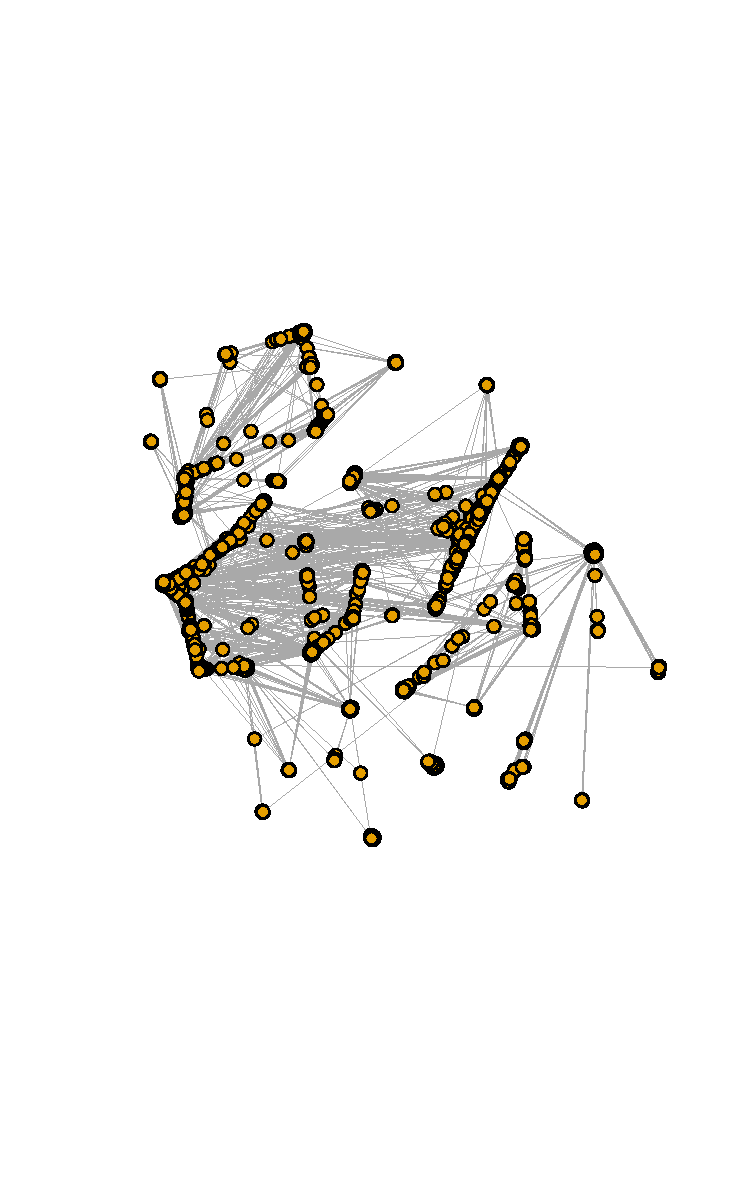
\includegraphics{figure/31fbelplot.pdf}
  \caption{Overview of our component of the Facebook network}
  \end{figure}
  
  \section{Generating Random Graphs}\label{generating-random-graphs}
  
  For each model, we created graphs of parable magnitude using some of the
  information calculated from the our Facebook network. We compared
  selected statistical network statistics of the Facebook network with
  that of the graphs we generate to see if the observed network and the
  simulated graphs have similar characteristics. We explain the process of
  generating one random graph for each model in the sections below. We
  simulated \(1000\) random graphs for each model and recorded the
  statistics such as transitivity, diameter, and average centrality
  values. Because we had \(1000\) values (one for each random graph for
  each model), we then recorded the average of these values. This means
  that for statistics such as average degree, we were interested in
  recording an average of the averages. The first column of
  \autoref{tab:erwsdescstats} shows the network statisitcs we were
  interested in and the average statistics recorded under each model as
  well as the standard deviation.
  
  \subsection{Using the Erdős-Rényi
  Model}\label{using-the-erdos-renyi-model}
  
  The Erdős-Rényi model only takes in two parameters, which are the number
  of nodes and the fixed probability of edge formation. The number of
  edges is already given as \(4039\), but to find the probability, we
  estimate this by taking the number of obsevred edges and divide it by
  the number of possible edges. For a graph \(G\), this estimated
  probability is
  
  \[\hat{p} = \frac {N_{E}} {{N_{V} \choose 2}}\]
  
  where \(N_{E}\) is the number of edges in \(G\), \(V_G\) is the number
  of nodes in \(G\).
  
  Thus, in order to simulate one graph from this model, we must look at
  each possible edge among the \(4039\) nodes and determine if an edge
  will form based on the given probability.
  
  \begin{Shaded}
  \begin{Highlighting}[]
  \KeywordTok{set.seed}\NormalTok{(}\DecValTok{499}\NormalTok{)}
  
  \NormalTok{numsim <-}\StringTok{ }\DecValTok{1000}
  
  \NormalTok{g.er.fbel.ecount <-}\StringTok{ }\KeywordTok{rep}\NormalTok{(}\OtherTok{NA}\NormalTok{, numsim)}
  \NormalTok{g.er.fbel.coef <-}\StringTok{ }\KeywordTok{rep}\NormalTok{(}\OtherTok{NA}\NormalTok{, numsim)}
  \NormalTok{g.er.fbel.apl <-}\StringTok{ }\KeywordTok{rep}\NormalTok{(}\OtherTok{NA}\NormalTok{, numsim)}
  \NormalTok{g.er.fbel.dia <-}\StringTok{ }\KeywordTok{rep}\NormalTok{(}\OtherTok{NA}\NormalTok{, numsim)}
  \NormalTok{g.er.fbel.avgdeg <-}\StringTok{ }\KeywordTok{rep}\NormalTok{(}\OtherTok{NA}\NormalTok{, numsim)}
  \NormalTok{g.er.fbel.avgbtwcen <-}\StringTok{ }\KeywordTok{rep}\NormalTok{(}\OtherTok{NA}\NormalTok{, numsim)}
  \NormalTok{g.er.fbel.avgclocen <-}\StringTok{ }\KeywordTok{rep}\NormalTok{(}\OtherTok{NA}\NormalTok{, numsim)}
  \NormalTok{g.er.fbel.avgeigveccen <-}\StringTok{ }\KeywordTok{rep}\NormalTok{(}\OtherTok{NA}\NormalTok{, numsim)}
  
  \CommentTok{#probability used in for-loop below}
  \NormalTok{p =}\StringTok{ }\KeywordTok{ecount}\NormalTok{(fbel)/}\KeywordTok{choose}\NormalTok{(}\KeywordTok{vcount}\NormalTok{(fbel), }\DecValTok{2}\NormalTok{)}
  
  \NormalTok{for (i in }\DecValTok{1}\NormalTok{:numsim) \{}
    \CommentTok{# n = number of vertices, p = probability of a link}
    \CommentTok{#p is caluclated as number of edges over number of possible edges}
    \CommentTok{#p is then (4039 choose 2) as calculated above }
    \CommentTok{#igraph object}
    \NormalTok{g.er.fbel <-}\StringTok{ }\KeywordTok{erdos.renyi.game}\NormalTok{(}\DataTypeTok{n =} \KeywordTok{vcount}\NormalTok{(fbel), p)}
    
    \CommentTok{#observe the network statistics for this simulated graph}
    \NormalTok{g.er.fbel.ecount[i] <-}\StringTok{ }\KeywordTok{ecount}\NormalTok{(g.er.fbel)}
    \NormalTok{g.er.fbel.coef[i] <-}\StringTok{ }\KeywordTok{transitivity}\NormalTok{(g.er.fbel, }\DataTypeTok{type=}\StringTok{"localaverage"}\NormalTok{)}
    \NormalTok{g.er.fbel.apl[i] <-}\StringTok{ }\KeywordTok{average.path.length}\NormalTok{(g.er.fbel)}
    \NormalTok{g.er.fbel.dia[i] <-}\StringTok{ }\KeywordTok{diameter}\NormalTok{(g.er.fbel)}
    \NormalTok{g.er.fbel.avgdeg[i] <-}\StringTok{ }\KeywordTok{mean}\NormalTok{(igraph::}\KeywordTok{degree}\NormalTok{(g.er.fbel))}
    \NormalTok{g.er.fbel.avgbtwcen[i] <-}\StringTok{ }\KeywordTok{mean}\NormalTok{(igraph::}\KeywordTok{betweenness}\NormalTok{(g.er.fbel))}
    \NormalTok{g.er.fbel.avgclocen[i] <-}\StringTok{ }\KeywordTok{mean}\NormalTok{(igraph::}\KeywordTok{closeness}\NormalTok{(g.er.fbel))}
    \NormalTok{g.er.fbel.avgeigveccen[i] <-}\StringTok{ }\KeywordTok{mean}\NormalTok{(igraph::}\KeywordTok{eigen_centrality}\NormalTok{(g.er.fbel)$vector)}
  \NormalTok{\}}
  
  \CommentTok{#save values as dataframe}
  \NormalTok{g.er.fbel <-}\StringTok{ }\KeywordTok{as.data.frame}\NormalTok{(}\KeywordTok{cbind}\NormalTok{(g.er.fbel.ecount, g.er.fbel.coef, }
                                   \NormalTok{g.er.fbel.apl, g.er.fbel.dia, }
                                   \NormalTok{g.er.fbel.avgdeg, g.er.fbel.avgbtwcen, }
                                   \NormalTok{g.er.fbel.avgclocen, g.er.fbel.avgeigveccen))}
  \end{Highlighting}
  \end{Shaded}
  
  \subsection{Using the Watts-Strogatz
  Model}\label{using-the-watts-strogatz-model}
  
  The Watts-Strogatz model takes in the following: the number of nodes
  \(N_{V}\), the number of starting neighbors \(r\), and the probability
  of an edge to be rewired \(p\). However, instead of rewiring our edges
  with a fixed probability, we will instead randomly add edges until we
  have approximately the same number as our observed network. To do this,
  we start with a lattice with \(4039\) nodes and assign a number of edges
  to the nodes equal to the smallest degree seen in our Facebook network
  (which we find to be \(1\)). This is our starting number of neighbors
  for each node. In this situation, \(p = 0\). We then randomly add edges
  equal to the difference between the our starting lattice and the
  observed network. That is, we add \(88234 - 4039 = 84195\) edges to our
  lattice. Finally, we simplify our simulated graph to eliminate
  multi-edges and loops. Since there are \(4039 \choose 2\) edges to
  choose from, intuitively, we can see that having many multi-edges or
  loops will be infrequent. This makes up one simulated graph from the
  model.
  
  \begin{Shaded}
  \begin{Highlighting}[]
  \KeywordTok{set.seed}\NormalTok{(}\DecValTok{499}\NormalTok{)}
  
  \NormalTok{numsim <-}\StringTok{ }\DecValTok{1000}
  
  \NormalTok{g.ws.fbel.ecount <-}\StringTok{ }\KeywordTok{rep}\NormalTok{(}\OtherTok{NA}\NormalTok{,numsim)}
  \NormalTok{g.ws.fbel.coef <-}\StringTok{ }\KeywordTok{rep}\NormalTok{(}\OtherTok{NA}\NormalTok{, numsim)}
  \NormalTok{g.ws.fbel.apl <-}\StringTok{ }\KeywordTok{rep}\NormalTok{(}\OtherTok{NA}\NormalTok{, numsim)}
  \NormalTok{g.ws.fbel.dia <-}\StringTok{ }\KeywordTok{rep}\NormalTok{(}\OtherTok{NA}\NormalTok{, numsim)}
  \NormalTok{g.ws.fbel.avgdeg <-}\StringTok{ }\KeywordTok{rep}\NormalTok{(}\OtherTok{NA}\NormalTok{, numsim)}
  \NormalTok{g.ws.fbel.avgbtwcen <-}\StringTok{ }\KeywordTok{rep}\NormalTok{(}\OtherTok{NA}\NormalTok{, numsim)}
  \NormalTok{g.ws.fbel.avgclocen <-}\StringTok{ }\KeywordTok{rep}\NormalTok{(}\OtherTok{NA}\NormalTok{, numsim)}
  \NormalTok{g.ws.fbel.avgeigveccen <-}\StringTok{ }\KeywordTok{rep}\NormalTok{(}\OtherTok{NA}\NormalTok{, numsim)}
  
  \NormalTok{for (i in }\DecValTok{1}\NormalTok{:numsim) \{}
    \CommentTok{#create a lattice with the same number of vertices as 'fbel'}
    \CommentTok{#let the starting number of neighbors be }
     \CommentTok{#equal to the minimum vertex degree of 'fbel'}
    \NormalTok{g.ws.fbel <-}\StringTok{ }\KeywordTok{watts.strogatz.game}\NormalTok{(}\DataTypeTok{dim =} \DecValTok{1}\NormalTok{, }\DataTypeTok{size =} \KeywordTok{vcount}\NormalTok{(fbel), }
                                     \DataTypeTok{nei =} \KeywordTok{min}\NormalTok{(}\KeywordTok{degree}\NormalTok{(fbg)), }\DataTypeTok{p =} \DecValTok{0}\NormalTok{)}
    
    \CommentTok{#generate list of random vertex values to add edges to lattice}
    \CommentTok{#each pair in the list represents one random edge}
    \NormalTok{randomedgepairs <-}\StringTok{ }\KeywordTok{sample}\NormalTok{(}\DecValTok{1}\NormalTok{:}\KeywordTok{vcount}\NormalTok{(fbel), }\DecValTok{2}\NormalTok{*(}\KeywordTok{ecount}\NormalTok{(fbel)-}\KeywordTok{vcount}\NormalTok{(fbel)), }
                              \DataTypeTok{replace=}\OtherTok{TRUE}\NormalTok{)}
    \NormalTok{g.ws.fbel.pre <-}\StringTok{ }\KeywordTok{add_edges}\NormalTok{(g.ws.fbel, randomedgepairs)}
      
    
    \CommentTok{#igraph object}
    \NormalTok{g.ws.fbel <-}\StringTok{ }\KeywordTok{simplify}\NormalTok{(g.ws.fbel.pre)}
    
    \CommentTok{#observe the network statistics for this simulated graph}
    \NormalTok{g.ws.fbel.ecount[i] <-}\StringTok{ }\KeywordTok{ecount}\NormalTok{(g.ws.fbel)}
    \NormalTok{g.ws.fbel.coef[i] <-}\StringTok{ }\KeywordTok{transitivity}\NormalTok{(g.ws.fbel, }\DataTypeTok{type=}\StringTok{"localaverage"}\NormalTok{)}
    \NormalTok{g.ws.fbel.apl[i] <-}\StringTok{ }\KeywordTok{average.path.length}\NormalTok{(g.ws.fbel)}
    \NormalTok{g.ws.fbel.dia[i] <-}\StringTok{ }\KeywordTok{diameter}\NormalTok{(g.ws.fbel)}
    \NormalTok{g.ws.fbel.avgdeg[i] <-}\StringTok{ }\KeywordTok{mean}\NormalTok{(igraph::}\KeywordTok{degree}\NormalTok{(g.ws.fbel))}
    \NormalTok{g.ws.fbel.avgbtwcen[i] <-}\StringTok{ }\KeywordTok{mean}\NormalTok{(igraph::}\KeywordTok{betweenness}\NormalTok{(g.ws.fbel))}
    \NormalTok{g.ws.fbel.avgclocen[i] <-}\StringTok{ }\KeywordTok{mean}\NormalTok{(igraph::}\KeywordTok{closeness}\NormalTok{(g.ws.fbel))}
    \NormalTok{g.ws.fbel.avgeigveccen[i] <-}\StringTok{ }\KeywordTok{mean}\NormalTok{(igraph::}\KeywordTok{eigen_centrality}\NormalTok{(g.ws.fbel)$vector)}
  \NormalTok{\}}
  
  \CommentTok{#save values as dataframe}
  \NormalTok{g.ws.fbel <-}\StringTok{ }\KeywordTok{as.data.frame}\NormalTok{(}\KeywordTok{cbind}\NormalTok{(g.ws.fbel.ecount, g.ws.fbel.coef, }
                                   \NormalTok{g.ws.fbel.apl, g.ws.fbel.dia, }
                                   \NormalTok{g.ws.fbel.avgdeg, g.ws.fbel.avgbtwcen, }
                                   \NormalTok{g.ws.fbel.avgclocen, g.ws.fbel.avgeigveccen))}
  \end{Highlighting}
  \end{Shaded}
  
  \subsection{Using ERGMs}\label{using-ergms}
  
  At the time of this writing, I am still currently working on the code
  for this section of the simulation study. A description of random graph
  construction and results, along with an associated code chuck will be
  included in the thesis submission of this project.
  
  \begin{Shaded}
  \begin{Highlighting}[]
  \CommentTok{#needs an object of class network}
  \CommentTok{#this should be the same as Erdős-Rényi}
  \NormalTok{g.ergm1.fbg <-}\StringTok{ }\KeywordTok{ergm}\NormalTok{(fbg ~}\StringTok{ }\NormalTok{edges)}
  
  \KeywordTok{set.seed}\NormalTok{(}\DecValTok{499}\NormalTok{)}
  \NormalTok{g.ergm1.fbg.sim <-}\StringTok{ }\KeywordTok{simulate}\NormalTok{(g.ergm1.fbg, }\DataTypeTok{numsim=}\DecValTok{1000}\NormalTok{)}
  
  
  
  \NormalTok{g.ergm2.fbg <-}\StringTok{ }\KeywordTok{ergm}\NormalTok{(fbg ~}\StringTok{ }\NormalTok{edges+triangle)}
  
  \KeywordTok{set.seed}\NormalTok{(}\DecValTok{499}\NormalTok{)}
  \NormalTok{g.ergm2.fbg.sim <-}\StringTok{ }\KeywordTok{simulate}\NormalTok{(g.ergm2.fbg, }\DataTypeTok{numsim=}\DecValTok{1000}\NormalTok{)}
  \end{Highlighting}
  \end{Shaded}
  
  \clearpage
  
  \begin{longtable}[]{@{}llll@{}}
  \caption{Comparisons of Network Statistics in among graphs simulated
  from classical graph models and the observed network
  \label{tab:erwsdescstats}}\tabularnewline
  \toprule
  \begin{minipage}[b]{0.29\columnwidth}\raggedright\strut
  Network Statistic\strut
  \end{minipage} & \begin{minipage}[b]{0.11\columnwidth}\raggedright\strut
  Observed\strut
  \end{minipage} & \begin{minipage}[b]{0.25\columnwidth}\raggedright\strut
  Erdős-Rényi\strut
  \end{minipage} & \begin{minipage}[b]{0.25\columnwidth}\raggedright\strut
  Watts-Strogatz\strut
  \end{minipage}\tabularnewline
  \midrule
  \endfirsthead
  \toprule
  \begin{minipage}[b]{0.29\columnwidth}\raggedright\strut
  Network Statistic\strut
  \end{minipage} & \begin{minipage}[b]{0.11\columnwidth}\raggedright\strut
  Observed\strut
  \end{minipage} & \begin{minipage}[b]{0.25\columnwidth}\raggedright\strut
  Erdős-Rényi\strut
  \end{minipage} & \begin{minipage}[b]{0.25\columnwidth}\raggedright\strut
  Watts-Strogatz\strut
  \end{minipage}\tabularnewline
  \midrule
  \endhead
  \begin{minipage}[t]{0.29\columnwidth}\raggedright\strut
  Transitivity\strut
  \end{minipage} & \begin{minipage}[t]{0.11\columnwidth}\raggedright\strut
  0.617\strut
  \end{minipage} & \begin{minipage}[t]{0.25\columnwidth}\raggedright\strut
  0.0108 \(\pm\) 0.0001\strut
  \end{minipage} & \begin{minipage}[t]{0.25\columnwidth}\raggedright\strut
  0.0107 \(\pm\) 9.135e-05\strut
  \end{minipage}\tabularnewline
  \begin{minipage}[t]{0.29\columnwidth}\raggedright\strut
  Average Path Length\strut
  \end{minipage} & \begin{minipage}[t]{0.11\columnwidth}\raggedright\strut
  4.338\strut
  \end{minipage} & \begin{minipage}[t]{0.25\columnwidth}\raggedright\strut
  2.606 \(\pm\) 0.002\strut
  \end{minipage} & \begin{minipage}[t]{0.25\columnwidth}\raggedright\strut
  2.6093 \(\pm\) 0.0002\strut
  \end{minipage}\tabularnewline
  \begin{minipage}[t]{0.29\columnwidth}\raggedright\strut
  Diameter\strut
  \end{minipage} & \begin{minipage}[t]{0.11\columnwidth}\raggedright\strut
  17\strut
  \end{minipage} & \begin{minipage}[t]{0.25\columnwidth}\raggedright\strut
  3.96 \(\pm\) 0.21\strut
  \end{minipage} & \begin{minipage}[t]{0.25\columnwidth}\raggedright\strut
  3.95 \(\pm\) 0.22\strut
  \end{minipage}\tabularnewline
  \begin{minipage}[t]{0.29\columnwidth}\raggedright\strut
  Average Degree\strut
  \end{minipage} & \begin{minipage}[t]{0.11\columnwidth}\raggedright\strut
  43.691\strut
  \end{minipage} & \begin{minipage}[t]{0.25\columnwidth}\raggedright\strut
  43.69 \(\pm\) 0.14\strut
  \end{minipage} & \begin{minipage}[t]{0.25\columnwidth}\raggedright\strut
  43.45 \(\pm\) 0.01\strut
  \end{minipage}\tabularnewline
  \begin{minipage}[t]{0.29\columnwidth}\raggedright\strut
  Average Betweenness Centrality\strut
  \end{minipage} & \begin{minipage}[t]{0.11\columnwidth}\raggedright\strut
  2072.642\strut
  \end{minipage} & \begin{minipage}[t]{0.25\columnwidth}\raggedright\strut
  3242 \(\pm\) 4\strut
  \end{minipage} & \begin{minipage}[t]{0.25\columnwidth}\raggedright\strut
  3249.2 \(\pm\) 0.4\strut
  \end{minipage}\tabularnewline
  \begin{minipage}[t]{0.29\columnwidth}\raggedright\strut
  Average Closeness Centrality\strut
  \end{minipage} & \begin{minipage}[t]{0.11\columnwidth}\raggedright\strut
  8.881e-08\strut
  \end{minipage} & \begin{minipage}[t]{0.25\columnwidth}\raggedright\strut
  9.507e-05 \(\pm\) 7.230e-08\strut
  \end{minipage} & \begin{minipage}[t]{0.25\columnwidth}\raggedright\strut
  9.494e-05 \(\pm\) 7.319e-09\strut
  \end{minipage}\tabularnewline
  \begin{minipage}[t]{0.29\columnwidth}\raggedright\strut
  Average Eigenvector Centrality\strut
  \end{minipage} & \begin{minipage}[t]{0.11\columnwidth}\raggedright\strut
  0.040\strut
  \end{minipage} & \begin{minipage}[t]{0.25\columnwidth}\raggedright\strut
  0.6202 \(\pm\) 0.0224\strut
  \end{minipage} & \begin{minipage}[t]{0.25\columnwidth}\raggedright\strut
  0.6235 \(\pm\) 0.0227\strut
  \end{minipage}\tabularnewline
  \bottomrule
  \end{longtable}
  
  Based on the results above, we see that the estimated average statistics
  for the Erdős-Rényi and Watts-Strogatz models are very similar to each
  other but are drastically different from many of the observed values of
  our Facebook network. This means that while the graphs generated from
  each model look very similar to each other, they look drastically
  different from our observed Facebook network. This is no surprise since
  the methods used to construct graphs under both models are very likely
  to generate almost the same number of verticles. We even see this in our
  simulation study; in the fourth row of \autoref{tab:erwsdescstats}, the
  average degree estimate for both models was within one degree from each
  other. Additionally, in both constructions, we are adding the edges
  randomly, so they are almost always spread evenly throughout the
  \(4039\) nodes. This means that additional features of the observed
  network, such as large clusters or degrees with high centralities, are
  likely to be missed by graphs generated from these two models. This is
  why the transitivity, average path length, and diameter for both models
  are smaller than what was actually observed. Similarly, because of how
  dispersed the edges are throughout the nodes, it is likely that there
  are many more nodes with higher centralities than in the observed
  network, making the average centrality measures for the graph models
  larger than those seen in the observed model. The only statistic whose
  value was actually close to, if not equal to, the observed value was the
  average degree. However, this makes sense since we fixed the probability
  \(p\) of a link forming in the Erdős-Rényi model (which of is directly
  proportional to the average degree) and because we ensured that every
  graph generated from the Watts-Strogatz model has about the same number
  of edges as the observed network. Thus, we have shown through this
  simulation study that the Erdős-Rényi and Watts-Strogatz models are not
  very accurate in modeling our Facebook network for these particular
  network statistics.
  
  \chapter*{Conclusion}\label{conclusion}
  \addcontentsline{toc}{chapter}{Conclusion}
  
  \setcounter{chapter}{4} \setcounter{section}{0}
  
  In this work, we have provided a brief overview of networks, network
  statistics, and graph models. We also applied certain graph models and
  fit them to our component of the Facebook network. By letting the graph
  models take in parameters that match those of our Facebook network, we
  generated graphs of parable magnitude. We compare the network statistics
  between these generated graphs and our target network to measure each
  model's accuracy. We showed through a simulation study that both the
  Erdős-Rényi and Watts-Strogatz models do not do a good job of modeling
  the Facebook network for particular network statistics.
  
  Over the next month, we will be creating ERGM models to fit the Facebook
  network and simulating from these models to see if the network
  statistics of these simulated graphs are closer to that of the observed
  network. As described in Chapter 3, once main advantage of ERGMs is that
  they allow for flexibility in model construction. This means we will be
  able to look at structures commonly seen in models and use them as
  parameters in ERGMs. This can include things such as k-stars (nodes with
  degree \(k\)), triangles, and distance, for example.
  
  This simulation study only scratches the surface of what network science
  has to offer. Firstly, we can bring in other social networks into this
  study. Could underlying undirected graphs of directed networks be better
  fit for the models here? Could network size be a factor as well? It is
  also possible for us to test other network statistics. Without providng
  the definitions, we can consider values such as \emph{reciprocity},
  \emph{assortivity}, or even other centrality measures. See Newman (2010)
  for more details. It is equally possible for us to choose other models
  to test our current Facebook network on. In fact, many other graphs
  models exist beyond what was presented here. Because social networks
  exhibit certain characteristics different from other kinds of networks,
  it comes as no surprise that there have been other models that are
  specifically tailored to its study. See Toivonen et al. (2009) for more
  a study of \emph{network evolution models} and \emph{nodal attribute
  models}, two specific types of social network models. Also, see Jurij
  Leskovec, Chakrabarti, Kleinberg, \& Faloutsos (2005) and Jure Leskovec,
  Chakrabarti, Kleinberg, Faloutsos, \& Ghahramani (2010) for an overview
  of networks in general and also recent developments in network science.
  They introduce \emph{Kronecker graphs} that have the benefit of only
  requiring a few parameters to fit to a target network in linear time. A
  successful simulation study has many implications that can benefit not
  only just network science, but all disciplines.
  
  \appendix
  
  \chapter{R/R-Markdown Code}\label{rr-markdown-code}
  
  This first appendix includes all of the R chunks of code used throughout
  the document (using the \texttt{include\ =\ FALSE} chunk tag) to help
  with readability and/or setup. Some code chunks were shown in the main
  body of the chapters for clarity and illustration.
  
  \subsubsection{In the main Rmd file:}\label{in-the-main-rmd-file}
  
  This is the setup file for the template.
  
  \begin{Shaded}
  \begin{Highlighting}[]
  \CommentTok{# This chunk ensures that the acstats package is}
  \CommentTok{# installed and loaded. This acstats package includes}
  \CommentTok{# the template files for the thesis and also two functions}
  \CommentTok{# used for labeling and referencing}
  \NormalTok{if(!}\KeywordTok{require}\NormalTok{(devtools))}
    \KeywordTok{install.packages}\NormalTok{(}\StringTok{"devtools"}\NormalTok{, }\DataTypeTok{repos =} \StringTok{"http://cran.rstudio.com"}\NormalTok{)}
  \NormalTok{if(!}\KeywordTok{require}\NormalTok{(acstats))\{}
    \KeywordTok{library}\NormalTok{(devtools)}
    \NormalTok{devtools::}\KeywordTok{install_github}\NormalTok{(}\StringTok{"Amherst-Statistics/acstats"}\NormalTok{)}
  \NormalTok{\}}
  \KeywordTok{library}\NormalTok{(acstats)}
  \end{Highlighting}
  \end{Shaded}
  
  The following are the packages used throughout this work. In particular,
  the \texttt{igraph}, \texttt{network}, \texttt{statnet}, and
  \texttt{ergm} packages were heavily used throughout all the chapters.
  
  \begin{Shaded}
  \begin{Highlighting}[]
  \KeywordTok{library}\NormalTok{(sand)}
  \KeywordTok{library}\NormalTok{(igraph)}
  \KeywordTok{library}\NormalTok{(network)}
  \KeywordTok{library}\NormalTok{(sna)}
  \KeywordTok{library}\NormalTok{(statnet)}
  \KeywordTok{library}\NormalTok{(ergm)}
  \KeywordTok{library}\NormalTok{(xtable)}
  
  \KeywordTok{options}\NormalTok{(}\DataTypeTok{xtable.comment =} \OtherTok{FALSE}\NormalTok{)}
  \KeywordTok{options}\NormalTok{(}\DataTypeTok{digits =} \DecValTok{4}\NormalTok{)}
  \end{Highlighting}
  \end{Shaded}
  
  \subsubsection{In Introduction}\label{in-introduction}
  
  We use the \texttt{karate} and \texttt{lawyer} data sets as examples to
  illustrate our discussion of networks.
  
  \begin{Shaded}
  \begin{Highlighting}[]
  \KeywordTok{data}\NormalTok{(karate)}
  \KeywordTok{data}\NormalTok{(lazega)}
  \end{Highlighting}
  \end{Shaded}
  
  The following code chunk generates a visual representing Zachary's
  karate club network.
  
  \begin{Shaded}
  \begin{Highlighting}[]
  \KeywordTok{plot}\NormalTok{(karate)}
  \end{Highlighting}
  \end{Shaded}
  
  The following code chunk generates a visual representing Lazega's law
  firm network.
  
  \begin{Shaded}
  \begin{Highlighting}[]
  \CommentTok{# Office location indicated by color.}
  \NormalTok{colbar <-}\StringTok{ }\KeywordTok{c}\NormalTok{(}\StringTok{"red"}\NormalTok{, }\StringTok{"dodgerblue"}\NormalTok{, }\StringTok{"goldenrod"}\NormalTok{)}
  \NormalTok{v.colors <-}\StringTok{ }\NormalTok{colbar[}\KeywordTok{V}\NormalTok{(lazega)$Office]}
  \CommentTok{# Type of practice indicated by vertex shape.}
  \NormalTok{v.shapes <-}\StringTok{ }\KeywordTok{c}\NormalTok{(}\StringTok{"circle"}\NormalTok{, }\StringTok{"square"}\NormalTok{)[}\KeywordTok{V}\NormalTok{(lazega)$Practice]}
  \CommentTok{# Vertex size proportional to years with firm.}
  \NormalTok{v.size <-}\StringTok{ }\FloatTok{3.5}\NormalTok{*}\KeywordTok{sqrt}\NormalTok{(}\KeywordTok{V}\NormalTok{(lazega)$Years)}
  \CommentTok{# Label vertices according to seniority.}
  \NormalTok{v.label <-}\StringTok{ }\KeywordTok{V}\NormalTok{(lazega)$Seniority}
  \CommentTok{# Reproducible layout.}
  \KeywordTok{set.seed}\NormalTok{(}\DecValTok{42}\NormalTok{)}
  \NormalTok{l <-}\StringTok{ }\KeywordTok{layout.fruchterman.reingold}\NormalTok{(lazega)}
  \KeywordTok{plot}\NormalTok{(lazega, }\DataTypeTok{layout=}\NormalTok{l, }\DataTypeTok{vertex.color=}\NormalTok{v.colors,}
       \DataTypeTok{vertex.shape=}\NormalTok{v.shapes, }\DataTypeTok{vertex.size=}\NormalTok{v.size,}
       \DataTypeTok{vertex.label=}\NormalTok{v.label)}
  \end{Highlighting}
  \end{Shaded}
  
  \subsubsection{In Chapter 1}\label{in-chapter-1}
  
  \begin{Shaded}
  \begin{Highlighting}[]
  \KeywordTok{mean}\NormalTok{(igraph::}\KeywordTok{degree}\NormalTok{(karate)) }
  \CommentTok{#average degree centrality: 4.588235}
  \KeywordTok{mean}\NormalTok{(igraph::}\KeywordTok{betweenness}\NormalTok{(karate)) }
  \CommentTok{#average betweenness centrality: 26.19363}
  \KeywordTok{mean}\NormalTok{(igraph::}\KeywordTok{closeness}\NormalTok{(karate)) }
  \CommentTok{#average closeness centrality: 0.005450958}
  \KeywordTok{mean}\NormalTok{(igraph::}\KeywordTok{eigen_centrality}\NormalTok{(karate)$vector) }
  \CommentTok{#average eigenvector centrality 0.3772814}
  
  \KeywordTok{mean}\NormalTok{(igraph::}\KeywordTok{degree}\NormalTok{(lazega)) }
  \CommentTok{#average degree centrality: 6.388889}
  \KeywordTok{mean}\NormalTok{(igraph::}\KeywordTok{betweenness}\NormalTok{(lazega)) }
  \CommentTok{#average betweenness centrality: 17.83333}
  \KeywordTok{mean}\NormalTok{(igraph::}\KeywordTok{closeness}\NormalTok{(lazega)) }
  \CommentTok{#average closeness centrality: 0.00670515}
  \KeywordTok{mean}\NormalTok{(igraph::}\KeywordTok{eigen_centrality}\NormalTok{(lazega)$vector) }
  \CommentTok{#average eigenvector centrality 0.4578719}
  \end{Highlighting}
  \end{Shaded}
  
  \subsubsection{In Chapter 2}\label{in-chapter-2}
  
  This generates two igraph objects from the Erdős-Rényi model with
  specified parameters--the number of nodes being 10 and probability of
  edge formating being 0.25.
  
  \begin{Shaded}
  \begin{Highlighting}[]
  \KeywordTok{set.seed}\NormalTok{(}\DecValTok{499}\NormalTok{)}
  
  \NormalTok{g1.er <-}\StringTok{ }\KeywordTok{erdos.renyi.game}\NormalTok{(}\DataTypeTok{n =} \DecValTok{10}\NormalTok{, }\DataTypeTok{p =} \FloatTok{0.25}\NormalTok{)}
  \NormalTok{g2.er <-}\StringTok{ }\KeywordTok{erdos.renyi.game}\NormalTok{(}\DataTypeTok{n =} \DecValTok{10}\NormalTok{, }\DataTypeTok{p =} \FloatTok{0.25}\NormalTok{)}
  \end{Highlighting}
  \end{Shaded}
  
  The following code plots the two graphs simulated from the Erdős-Rényi
  model.
  
  \begin{Shaded}
  \begin{Highlighting}[]
  \KeywordTok{par}\NormalTok{(}\DataTypeTok{mfrow=}\KeywordTok{c}\NormalTok{(}\DecValTok{1}\NormalTok{,}\DecValTok{2}\NormalTok{))}
  \KeywordTok{plot}\NormalTok{(g1.er, }\DataTypeTok{vertex.size=}\DecValTok{20}\NormalTok{, }\DataTypeTok{vertex.label.cex =} \FloatTok{0.75}\NormalTok{)}
  \KeywordTok{plot}\NormalTok{(g2.er, }\DataTypeTok{vertex.size=}\DecValTok{20}\NormalTok{, }\DataTypeTok{vertex.label.cex =} \FloatTok{0.75}\NormalTok{)}
  \end{Highlighting}
  \end{Shaded}
  
  This generates two igraph objects from the Watts-Strogatz model with
  specified parameters--the number of nodes being 10, number of neighbors
  being 2, and probabilities 0 (left) and 0.25 (right).
  
  \begin{Shaded}
  \begin{Highlighting}[]
  \KeywordTok{set.seed}\NormalTok{(}\DecValTok{499}\NormalTok{)}
  
  \NormalTok{g1.ws <-}\StringTok{ }\KeywordTok{watts.strogatz.game}\NormalTok{(}\DataTypeTok{dim =} \DecValTok{1}\NormalTok{, }\DataTypeTok{size =} \DecValTok{10}\NormalTok{, }\DataTypeTok{nei =} \DecValTok{2}\NormalTok{, }\DataTypeTok{p =} \DecValTok{0}\NormalTok{)}
  \NormalTok{g2.ws <-}\StringTok{ }\KeywordTok{watts.strogatz.game}\NormalTok{(}\DataTypeTok{dim =} \DecValTok{1}\NormalTok{, }\DataTypeTok{size =} \DecValTok{10}\NormalTok{, }\DataTypeTok{nei =} \DecValTok{2}\NormalTok{, }\DataTypeTok{p =} \FloatTok{0.25}\NormalTok{)}
  \end{Highlighting}
  \end{Shaded}
  
  The following code plots the two graphs simulated from the
  Watts-Strogatz model.
  
  \begin{Shaded}
  \begin{Highlighting}[]
  \KeywordTok{par}\NormalTok{(}\DataTypeTok{mfrow=}\KeywordTok{c}\NormalTok{(}\DecValTok{1}\NormalTok{,}\DecValTok{2}\NormalTok{))}
  \KeywordTok{plot}\NormalTok{(g1.ws, }\DataTypeTok{vertex.size=}\DecValTok{20}\NormalTok{, }\DataTypeTok{vertex.label.cex =} \FloatTok{0.75}\NormalTok{)}
  \KeywordTok{plot}\NormalTok{(g2.ws, }\DataTypeTok{vertex.size=}\DecValTok{20}\NormalTok{, }\DataTypeTok{vertex.label.cex =} \FloatTok{0.75}\NormalTok{)}
  \end{Highlighting}
  \end{Shaded}
  
  \subsubsection{In Chapter 3}\label{in-chapter-3}
  
  We load in our Facebook data set, that is, our observed network. It is a
  simple, undiected, connected component of the network in the form of an
  edge list. We convert to an \texttt{igraph} object in order to calculate
  certain network statistics.
  
  \begin{Shaded}
  \begin{Highlighting}[]
  \KeywordTok{setwd}\NormalTok{(}\StringTok{"~/STAT495-Lee/LeeThesis/data"}\NormalTok{)}
  
  \CommentTok{#edge list}
  \NormalTok{facebookcombined <-}\StringTok{ }\KeywordTok{read.table}\NormalTok{(}\KeywordTok{gzfile}\NormalTok{(}\StringTok{"facebook_combined.txt.gz"}\NormalTok{), }\DataTypeTok{header=}\NormalTok{F)}
  
  \CommentTok{#igraph object}
  \NormalTok{fbel <-}\StringTok{ }\KeywordTok{graph.data.frame}\NormalTok{(facebookcombined)}
  \end{Highlighting}
  \end{Shaded}
  
  Below are some numbers (and the associated code for it) that
  characterize the observed Facebook network as well as some associated
  descriptive statistics.
  
  \begin{Shaded}
  \begin{Highlighting}[]
  \KeywordTok{length}\NormalTok{(}\KeywordTok{unique}\NormalTok{(}\KeywordTok{c}\NormalTok{(facebookcombined$V2, facebookcombined$V1))); }\KeywordTok{vcount}\NormalTok{(fbel)}
  \CommentTok{#number of vertices: 4039}
  \KeywordTok{nrow}\NormalTok{(facebookcombined); }\KeywordTok{ecount}\NormalTok{(fbel)}
  \CommentTok{#number of edges: 88234}
  \KeywordTok{sum}\NormalTok{(}\KeywordTok{count_triangles}\NormalTok{(fbel))/}\DecValTok{3} 
  \CommentTok{#number of unique triangles (up to ordering): 1612010}
  
  \KeywordTok{transitivity}\NormalTok{(fbel, }\DataTypeTok{type=}\StringTok{"localaverage"}\NormalTok{) }\CommentTok{#0.6170038}
  \KeywordTok{diameter}\NormalTok{(fbel) }\CommentTok{#17}
  \KeywordTok{average.path.length}\NormalTok{(fbel) }\CommentTok{#4.337744}
  
  \KeywordTok{mean}\NormalTok{(igraph::}\KeywordTok{degree}\NormalTok{(fbel)) }
  \CommentTok{#average degree centrality: 43.69101}
  \KeywordTok{mean}\NormalTok{(igraph::}\KeywordTok{betweenness}\NormalTok{(fbel)) }
  \CommentTok{#average betweenness centrality: 2072.642}
  \KeywordTok{mean}\NormalTok{(igraph::}\KeywordTok{closeness}\NormalTok{(fbel)) }
  \CommentTok{#average closeness centrality: 8.881448e-08}
  \KeywordTok{mean}\NormalTok{(igraph::}\KeywordTok{eigen_centrality}\NormalTok{(fbel)$vector) }
  \CommentTok{#average eigenvector centrality 0.04047316}
  \end{Highlighting}
  \end{Shaded}
  
  The code below plots the entire component of the Facebook that SNAP has
  provided.
  
  \begin{Shaded}
  \begin{Highlighting}[]
  \KeywordTok{plot}\NormalTok{(fbel, }
       \DataTypeTok{edge.arrow.size =} \DecValTok{0}\NormalTok{, }
       \DataTypeTok{edge.width =} \FloatTok{0.05}\NormalTok{, }
       \DataTypeTok{vertex.label =} \OtherTok{NA}\NormalTok{, }
       \DataTypeTok{vertex.size =} \DecValTok{5}\NormalTok{)}
  \end{Highlighting}
  \end{Shaded}
  
  The following code describes the data simulation process using the
  Erdős-Rényi model. We create seven empty vectors and fill the \(i^{th}\)
  term of each vector by running through a for loop that calculates seven
  network statisitcs for the \(i^{th}\) random graph generated from the
  model.
  
  \begin{Shaded}
  \begin{Highlighting}[]
  \KeywordTok{set.seed}\NormalTok{(}\DecValTok{499}\NormalTok{)}
  
  \NormalTok{numsim <-}\StringTok{ }\DecValTok{1000}
  
  \NormalTok{g.er.fbel.ecount <-}\StringTok{ }\KeywordTok{rep}\NormalTok{(}\OtherTok{NA}\NormalTok{, numsim)}
  \NormalTok{g.er.fbel.coef <-}\StringTok{ }\KeywordTok{rep}\NormalTok{(}\OtherTok{NA}\NormalTok{, numsim)}
  \NormalTok{g.er.fbel.apl <-}\StringTok{ }\KeywordTok{rep}\NormalTok{(}\OtherTok{NA}\NormalTok{, numsim)}
  \NormalTok{g.er.fbel.dia <-}\StringTok{ }\KeywordTok{rep}\NormalTok{(}\OtherTok{NA}\NormalTok{, numsim)}
  \NormalTok{g.er.fbel.avgdeg <-}\StringTok{ }\KeywordTok{rep}\NormalTok{(}\OtherTok{NA}\NormalTok{, numsim)}
  \NormalTok{g.er.fbel.avgbtwcen <-}\StringTok{ }\KeywordTok{rep}\NormalTok{(}\OtherTok{NA}\NormalTok{, numsim)}
  \NormalTok{g.er.fbel.avgclocen <-}\StringTok{ }\KeywordTok{rep}\NormalTok{(}\OtherTok{NA}\NormalTok{, numsim)}
  \NormalTok{g.er.fbel.avgeigveccen <-}\StringTok{ }\KeywordTok{rep}\NormalTok{(}\OtherTok{NA}\NormalTok{, numsim)}
  
  \CommentTok{#probability used in for-loop below}
  \NormalTok{p =}\StringTok{ }\KeywordTok{ecount}\NormalTok{(fbel)/}\KeywordTok{choose}\NormalTok{(}\KeywordTok{vcount}\NormalTok{(fbel), }\DecValTok{2}\NormalTok{)}
  
  \NormalTok{for (i in }\DecValTok{1}\NormalTok{:numsim) \{}
    \CommentTok{# n = number of vertices, p = probability of a link}
    \CommentTok{#p is caluclated as number of edges over number of possible edges}
    \CommentTok{#p is then (4039 choose 2) as calculated above }
    \CommentTok{#igraph object}
    \NormalTok{g.er.fbel <-}\StringTok{ }\KeywordTok{erdos.renyi.game}\NormalTok{(}\DataTypeTok{n =} \KeywordTok{vcount}\NormalTok{(fbel), p)}
    
    \CommentTok{#observe the network statistics for this simulated graph}
    \NormalTok{g.er.fbel.ecount[i] <-}\StringTok{ }\KeywordTok{ecount}\NormalTok{(g.er.fbel)}
    \NormalTok{g.er.fbel.coef[i] <-}\StringTok{ }\KeywordTok{transitivity}\NormalTok{(g.er.fbel, }\DataTypeTok{type=}\StringTok{"localaverage"}\NormalTok{)}
    \NormalTok{g.er.fbel.apl[i] <-}\StringTok{ }\KeywordTok{average.path.length}\NormalTok{(g.er.fbel)}
    \NormalTok{g.er.fbel.dia[i] <-}\StringTok{ }\KeywordTok{diameter}\NormalTok{(g.er.fbel)}
    \NormalTok{g.er.fbel.avgdeg[i] <-}\StringTok{ }\KeywordTok{mean}\NormalTok{(igraph::}\KeywordTok{degree}\NormalTok{(g.er.fbel))}
    \NormalTok{g.er.fbel.avgbtwcen[i] <-}\StringTok{ }\KeywordTok{mean}\NormalTok{(igraph::}\KeywordTok{betweenness}\NormalTok{(g.er.fbel))}
    \NormalTok{g.er.fbel.avgclocen[i] <-}\StringTok{ }\KeywordTok{mean}\NormalTok{(igraph::}\KeywordTok{closeness}\NormalTok{(g.er.fbel))}
    \NormalTok{g.er.fbel.avgeigveccen[i] <-}\StringTok{ }\KeywordTok{mean}\NormalTok{(igraph::}\KeywordTok{eigen_centrality}\NormalTok{(g.er.fbel)$vector)}
  \NormalTok{\}}
  
  \CommentTok{#save values as dataframe}
  \NormalTok{g.er.fbel <-}\StringTok{ }\KeywordTok{as.data.frame}\NormalTok{(}\KeywordTok{cbind}\NormalTok{(g.er.fbel.ecount, g.er.fbel.coef, }
                                   \NormalTok{g.er.fbel.apl, g.er.fbel.dia, }
                                   \NormalTok{g.er.fbel.avgdeg, g.er.fbel.avgbtwcen, }
                                   \NormalTok{g.er.fbel.avgclocen, g.er.fbel.avgeigveccen))}
  \end{Highlighting}
  \end{Shaded}
  
  The following code describes the data simulation process using the
  Watts-Strogatz model. This process is analogous to the process described
  above.
  
  \begin{Shaded}
  \begin{Highlighting}[]
  \KeywordTok{set.seed}\NormalTok{(}\DecValTok{499}\NormalTok{)}
  
  \NormalTok{numsim <-}\StringTok{ }\DecValTok{1000}
  
  \NormalTok{g.ws.fbel.ecount <-}\StringTok{ }\KeywordTok{rep}\NormalTok{(}\OtherTok{NA}\NormalTok{,numsim)}
  \NormalTok{g.ws.fbel.coef <-}\StringTok{ }\KeywordTok{rep}\NormalTok{(}\OtherTok{NA}\NormalTok{, numsim)}
  \NormalTok{g.ws.fbel.apl <-}\StringTok{ }\KeywordTok{rep}\NormalTok{(}\OtherTok{NA}\NormalTok{, numsim)}
  \NormalTok{g.ws.fbel.dia <-}\StringTok{ }\KeywordTok{rep}\NormalTok{(}\OtherTok{NA}\NormalTok{, numsim)}
  \NormalTok{g.ws.fbel.avgdeg <-}\StringTok{ }\KeywordTok{rep}\NormalTok{(}\OtherTok{NA}\NormalTok{, numsim)}
  \NormalTok{g.ws.fbel.avgbtwcen <-}\StringTok{ }\KeywordTok{rep}\NormalTok{(}\OtherTok{NA}\NormalTok{, numsim)}
  \NormalTok{g.ws.fbel.avgclocen <-}\StringTok{ }\KeywordTok{rep}\NormalTok{(}\OtherTok{NA}\NormalTok{, numsim)}
  \NormalTok{g.ws.fbel.avgeigveccen <-}\StringTok{ }\KeywordTok{rep}\NormalTok{(}\OtherTok{NA}\NormalTok{, numsim)}
  
  \NormalTok{for (i in }\DecValTok{1}\NormalTok{:numsim) \{}
    \CommentTok{#create a lattice with the same number of vertices as 'fbel'}
    \CommentTok{#let the starting number of neighbors be }
     \CommentTok{#equal to the minimum vertex degree of 'fbel'}
    \NormalTok{g.ws.fbel <-}\StringTok{ }\KeywordTok{watts.strogatz.game}\NormalTok{(}\DataTypeTok{dim =} \DecValTok{1}\NormalTok{, }\DataTypeTok{size =} \KeywordTok{vcount}\NormalTok{(fbel), }
                                     \DataTypeTok{nei =} \KeywordTok{min}\NormalTok{(}\KeywordTok{degree}\NormalTok{(fbg)), }\DataTypeTok{p =} \DecValTok{0}\NormalTok{)}
    
    \CommentTok{#generate list of random vertex values to add edges to lattice}
    \CommentTok{#each pair in the list represents one random edge}
    \NormalTok{randomedgepairs <-}\StringTok{ }\KeywordTok{sample}\NormalTok{(}\DecValTok{1}\NormalTok{:}\KeywordTok{vcount}\NormalTok{(fbel), }\DecValTok{2}\NormalTok{*(}\KeywordTok{ecount}\NormalTok{(fbel)-}\KeywordTok{vcount}\NormalTok{(fbel)), }
                              \DataTypeTok{replace=}\OtherTok{TRUE}\NormalTok{)}
    \NormalTok{g.ws.fbel.pre <-}\StringTok{ }\KeywordTok{add_edges}\NormalTok{(g.ws.fbel, randomedgepairs)}
      
    
    \CommentTok{#igraph object}
    \NormalTok{g.ws.fbel <-}\StringTok{ }\KeywordTok{simplify}\NormalTok{(g.ws.fbel.pre)}
    
    \CommentTok{#observe the network statistics for this simulated graph}
    \NormalTok{g.ws.fbel.ecount[i] <-}\StringTok{ }\KeywordTok{ecount}\NormalTok{(g.ws.fbel)}
    \NormalTok{g.ws.fbel.coef[i] <-}\StringTok{ }\KeywordTok{transitivity}\NormalTok{(g.ws.fbel, }\DataTypeTok{type=}\StringTok{"localaverage"}\NormalTok{)}
    \NormalTok{g.ws.fbel.apl[i] <-}\StringTok{ }\KeywordTok{average.path.length}\NormalTok{(g.ws.fbel)}
    \NormalTok{g.ws.fbel.dia[i] <-}\StringTok{ }\KeywordTok{diameter}\NormalTok{(g.ws.fbel)}
    \NormalTok{g.ws.fbel.avgdeg[i] <-}\StringTok{ }\KeywordTok{mean}\NormalTok{(igraph::}\KeywordTok{degree}\NormalTok{(g.ws.fbel))}
    \NormalTok{g.ws.fbel.avgbtwcen[i] <-}\StringTok{ }\KeywordTok{mean}\NormalTok{(igraph::}\KeywordTok{betweenness}\NormalTok{(g.ws.fbel))}
    \NormalTok{g.ws.fbel.avgclocen[i] <-}\StringTok{ }\KeywordTok{mean}\NormalTok{(igraph::}\KeywordTok{closeness}\NormalTok{(g.ws.fbel))}
    \NormalTok{g.ws.fbel.avgeigveccen[i] <-}\StringTok{ }\KeywordTok{mean}\NormalTok{(igraph::}\KeywordTok{eigen_centrality}\NormalTok{(g.ws.fbel)$vector)}
  \NormalTok{\}}
  
  \CommentTok{#save values as dataframe}
  \NormalTok{g.ws.fbel <-}\StringTok{ }\KeywordTok{as.data.frame}\NormalTok{(}\KeywordTok{cbind}\NormalTok{(g.ws.fbel.ecount, g.ws.fbel.coef, }
                                   \NormalTok{g.ws.fbel.apl, g.ws.fbel.dia, }
                                   \NormalTok{g.ws.fbel.avgdeg, g.ws.fbel.avgbtwcen, }
                                   \NormalTok{g.ws.fbel.avgclocen, g.ws.fbel.avgeigveccen))}
  \end{Highlighting}
  \end{Shaded}
  
  The following code descibes how to fit graphs using ERGMs and simulating
  from the models that have been constructed.
  
  \begin{Shaded}
  \begin{Highlighting}[]
  \CommentTok{#needs an object of class network}
  \CommentTok{#this should be the same as Erdős-Rényi}
  \NormalTok{g.ergm1.fbg <-}\StringTok{ }\KeywordTok{ergm}\NormalTok{(fbg ~}\StringTok{ }\NormalTok{edges)}
  
  \KeywordTok{set.seed}\NormalTok{(}\DecValTok{499}\NormalTok{)}
  \NormalTok{g.ergm1.fbg.sim <-}\StringTok{ }\KeywordTok{simulate}\NormalTok{(g.ergm1.fbg, }\DataTypeTok{numsim=}\DecValTok{1000}\NormalTok{)}
  
  
  
  \NormalTok{g.ergm2.fbg <-}\StringTok{ }\KeywordTok{ergm}\NormalTok{(fbg ~}\StringTok{ }\NormalTok{edges+triangle)}
  
  \KeywordTok{set.seed}\NormalTok{(}\DecValTok{499}\NormalTok{)}
  \NormalTok{g.ergm2.fbg.sim <-}\StringTok{ }\KeywordTok{simulate}\NormalTok{(g.ergm2.fbg, }\DataTypeTok{numsim=}\DecValTok{1000}\NormalTok{)}
  \end{Highlighting}
  \end{Shaded}
  
  \subsubsection{In Conclusion}\label{in-conclusion}
  
  None
  
  \backmatter
  
  \chapter{References}\label{references}
  
  \noindent
  
  \setlength{\parindent}{-0.20in} \setlength{\leftskip}{0.20in}
  \setlength{\parskip}{8pt}
  
  \hypertarget{refs}{}
  \hypertarget{ref-baumer_modern_2017}{}
  Baumer, B., Kaplan, D., \& Horton, N. (2017). \emph{Modern Data Science
  With R: With Digital Download}. Taylor \& Francis. Retrieved from
  \url{https://books.google.com/books?id=Gv1nvgAACAAJ}
  
  \hypertarget{ref-intergraphpackagemanual}{}
  Bojanowski, M. (2015). \emph{Intergraph: Coercion routines for network
  data objects}. Retrieved from \url{http://mbojan.github.io/intergraph}
  
  \hypertarget{ref-networkpackagearticle}{}
  Butts, C. T. (2008). Network: A package for managing relational data in
  r. \emph{Journal of Statistical Software}, \emph{24}(2). Retrieved from
  \url{http://www.jstatsoft.org/v24/i02/paper}
  
  \hypertarget{ref-networkpackagemanual}{}
  Butts, C. T. (2015). \emph{Network: Classes for relational data}. The
  Statnet Project (\url{http://statnet.org}). Retrieved from
  \url{http://CRAN.R-project.org/package=network}
  
  \hypertarget{ref-butts2008social}{}
  Butts, C. T., \& others. (2008). Social network analysis with sna.
  \emph{Journal of Statistical Software}, \emph{24}(6), 1--51.
  
  \hypertarget{ref-butts_introduction_2015}{}
  Butts, C., Hunter, D., Handcock, M. S., Morris, M., Krivtisky, P. N.,
  Almquist, Z., \ldots{} Bender de-Moll, S. (2015, June). Introduction to
  Exponential-family Random Graph (ERG or p*) modeling with ergm.
  Retrieved from
  \url{https://statnet.org/trac/raw-attachment/wiki/Sunbelt2015/ergm_tutorial.pdf}
  
  \hypertarget{ref-igraphpackage}{}
  Csárdi, G., \& Nepusz, T. (2006). The igraph software package for
  complex network research. \emph{InterJournal}, \emph{Complex Systems},
  1695. Retrieved from \url{http://igraph.org}
  
  \hypertarget{ref-erdos1959random}{}
  Erd\H{o}s, P., \& Rényi, A. (1959). On random graphs, i.
  \emph{Publicationes Mathematicae (Debrecen)}, \emph{6}, 290--297.
  
  \hypertarget{ref-erdos1960evolution}{}
  Erd\H{o}s, P., \& Rényi, A. (1960). On the evolution of random graphs.
  \emph{Publ. Math. Inst. Hung. Acad. Sci}, \emph{5}(1), 17--60.
  
  \hypertarget{ref-erdHos1964strength}{}
  Erd\H{o}s, P., \& Rényi, A. (1964). On the strength of connectedness of
  a random graph. \emph{Acta Mathematica Academiae Scientiarum Hungarica},
  \emph{12}(1-2), 261--267.
  
  \hypertarget{ref-gilbert1959random}{}
  Gilbert, E. N. (1959). Random graphs. \emph{The Annals of Mathematical
  Statistics}, \emph{30}(4), 1141--1144.
  
  \hypertarget{ref-statnetpackagearticle}{}
  Handcock, M. S., Hunter, D. R., Butts, C. T., Goodreau, S. M., \&
  Morris, M. (2008). Statnet: Software tools for the representation,
  visualization, analysis and simulation of network data. \emph{Journal of
  Statistical Software}, \emph{24}(1), 1--11. Retrieved from
  \url{http://www.jstatsoft.org/v24/i01}
  
  \hypertarget{ref-ergmpackagemanual}{}
  Handcock, M. S., Hunter, D. R., Butts, C. T., Goodreau, S. M.,
  Krivitsky, P. N., \& Morris, M. (2017). \emph{Ergm: Fit, simulate and
  diagnose exponential-family models for networks}. The Statnet Project
  (\url{http://www.statnet.org}). Retrieved from
  \url{https://CRAN.R-project.org/package=ergm}
  
  \hypertarget{ref-statnetpackagemanual}{}
  Handcock, M. S., Hunter, D. R., Butts, C. T., Goodreau, S. M.,
  Krivitsky, P. N., Bender-deMoll, S., \& Morris, M. (2016).
  \emph{Statnet: Software tools for the statistical analysis of network
  data}. The Statnet Project (\url{http://www.statnet.org}). Retrieved
  from \url{CRAN.R-project.org/package=statnet}
  
  \hypertarget{ref-ergmpackagearticle}{}
  Hunter, D. R., Handcock, M. S., Butts, C. T., Goodreau, S. M., Morris,
  \& Martina. (2008). Ergm: A package to fit, simulate and diagnose
  exponential-family models for networks. \emph{Journal of Statistical
  Software}, \emph{24}(3), 1--29.
  
  \hypertarget{ref-kolaczyk_statistical_2009}{}
  Kolaczyk, E. D. (2009). \emph{Statistical Analysis of Network Data:
  Methods and Models}. Springer Science \& Business Media.
  
  \hypertarget{ref-lazega1999multiplexity}{}
  Lazega, E., \& Pattison, P. E. (1999). Multiplexity, generalized
  exchange and cooperation in organizations: A case study. \emph{Social
  Networks}, \emph{21}(1), 67--90.
  
  \hypertarget{ref-snapnets}{}
  Leskovec, J., \& Krevl, A. (2014, June). SNAP Datasets: Stanford large
  network dataset collection. \url{http://snap.stanford.edu/data}.
  
  \hypertarget{ref-leskovec_realistic_2005}{}
  Leskovec, J., Chakrabarti, D., Kleinberg, J., \& Faloutsos, C. (2005).
  Realistic, Mathematically Tractable Graph Generation and Evolution,
  Using Kronecker Multiplication. In \emph{Knowledge Discovery in
  Databases: PKDD 2005} (pp. 133--145). Springer, Berlin, Heidelberg.
  Retrieved from
  \url{http://link.springer.com/chapter/10.1007/11564126_17}
  
  \hypertarget{ref-leskovec_kronecker_2010}{}
  Leskovec, J., Chakrabarti, D., Kleinberg, J., Faloutsos, C., \&
  Ghahramani, Z. (2010). Kronecker Graphs: An Approach to Modeling
  Networks. \emph{Journal of Machine Learning Research}, \emph{11}(Feb),
  985--1042. Retrieved from
  \url{http://www.jmlr.org/papers/v11/leskovec10a.html}
  
  \hypertarget{ref-newman_networks:_2010}{}
  Newman, M. (2010). \emph{Networks: An Introduction}. OUP Oxford.
  
  \hypertarget{ref-toivonen_comparative_2009}{}
  Toivonen, R., Kovanen, L., Kivelä, M., Onnela, J.-P., Saramäki, J., \&
  Kaski, K. (2009). A comparative study of social network models: Network
  evolution models and nodal attribute models. \emph{Social Networks},
  \emph{31}(4), 240--254.
  \url{http://doi.org/10.1016/j.socnet.2009.06.004}
  
  \hypertarget{ref-travers1967small}{}
  Travers, J., \& Milgram, S. (1967). The small world problem.
  \emph{Phychology Today}, \emph{1}, 61--67.
  
  \hypertarget{ref-watts_collective_1998}{}
  Watts, D. J., \& Strogatz, S. H. (1998). Collective dynamics of
  ``small-world'' networks. \emph{Nature}, \emph{393}(6684), 440--442.
  \url{http://doi.org/10.1038/30918}
  
  \hypertarget{ref-zachskarateclub}{}
  Zachary, W. W. (1977). An information flow model for conflict and
  fission in small groups. \emph{Journal of Anthropological Research},
  \emph{33}(4), 452--473. \url{http://doi.org/10.1086/jar.33.4.3629752}


  % Index?

\end{document}

